\chapter{Medicina de Sistemas}
\label{cap:13}

\normalfont\rmfamily\upshape
A medicina do século XX foi, em larga medida, uma medicina de alvos. Identificava-se uma molécula --- usualmente um receptor, uma enzima ou um canal iônico --- e projetava-se um composto para modulá-la. A doença aparecia, no modelo mental dominante, como consequência de uma alteração discreta em um componente bem definido, e a terapêutica seguia essa lógica: uma patologia, um alvo, um fármaco. Esse esquema produziu resultados extraordinários ao longo do século, da antibioticoterapia à quimioterapia antineoplásica, e permanece como a espinha dorsal da farmacologia clínica. Sua limitação, no entanto, tornou-se cada vez mais evidente à medida que as doenças remanescentes --- cardiovasculares, neurodegenerativas, metabólicas, oncológicas refratárias --- revelaram-se refratárias à estratégia de alvo único. Taxas de falha superiores a noventa por cento em ensaios clínicos, custos bilionários por fármaco aprovado e a recorrência quase inevitável de resistência tumoral e bacteriana sinalizaram que o paradigma precisava ser repensado. Esse repensar é o que se convencionou chamar de \emph{medicina de sistemas}: uma abordagem que trata a doença como fenômeno emergente de uma rede molecular, e a terapêutica como uma intervenção planejada sobre essa rede.

A ideia central é simples na formulação e profunda nas consequências. Em vez de buscar o ``gene da doença'' ou a ``proteína da doença'', a medicina de sistemas busca o \emph{módulo} da doença --- um conjunto de componentes topologicamente próximos no interactoma cujas perturbações, em conjunto, produzem um fenótipo patológico. Esse módulo não substitui o conceito clássico de patologia: um quadro clínico continua a ser descrito em termos de sintomas e sinais. O que muda é a camada explicativa subjacente. Quando se compreende que uma doença cardíaca resulta da interação entre variantes genéticas em dezenas de loci, perfis lipídicos individuais, inflamação crônica de baixo grau, função endotelial, coagulação e controle autonômico --- todos mediados por redes de centenas a milhares de proteínas ---, torna-se evidente que nenhuma intervenção pontual será suficiente para revertê-la de forma estável. O mesmo raciocínio aplica-se ao diabetes tipo 2, às doenças neurodegenerativas, à maioria dos cânceres sólidos e às doenças autoimunes. A complexidade não é ruído a ser removido; é a estrutura do problema.

A medicina personalizada e a medicina de precisão surgem, nesse contexto, como duas faces de uma mesma mudança de paradigma. A medicina tradicional --- aquela que o clínico aprende nos manuais e pratica nas enfermarias --- opera com protocolos estatísticos derivados de populações: a dose padrão de um anti-hipertensivo, o esquema padrão de uma poliquimioterapia, o ponto de corte de um biomarcador sérico. Esses protocolos são necessários e úteis, mas embutem uma assimetria informacional --- o paciente médio é uma abstração, e o paciente real está em algum lugar da distribuição, nem sempre próximo da média. A medicina personalizada, ao contrário, busca incorporar ao processo decisório a informação molecular individual: o genótipo do paciente para enzimas metabolizadoras, o perfil transcriptômico do tumor, a presença ou ausência de variantes driver específicas, a assinatura imune do microambiente tumoral. A decisão terapêutica deixa de ser aplicada a uma classe estatística e passa a ser otimizada para um indivíduo. \emph{O tratamento certo, para o paciente certo, no momento certo} --- o slogan da medicina personalizada --- é mais do que retórica: é a tradução operacional da ideia de que variabilidade biológica individual importa.

Este capítulo atravessa quatro domínios em que a biologia de sistemas se encontra com a prática médica contemporânea. A primeira seção trata da descoberta e do desenvolvimento de fármacos sob a ótica sistêmica: como as redes biológicas reconfiguram a identificação de alvos, como a farmacologia de redes substitui a lógica de um fármaco-um alvo, como a farmacocinética e a farmacodinâmica se formalizam em modelos matemáticos que permitem prever concentrações e efeitos, e como os ensaios clínicos incorporam estratificação molecular. A segunda seção aborda as doenças complexas --- câncer, doenças cardiovasculares, diabetes, doenças neurodegenerativas --- mostrando como cada uma delas é hoje compreendida como manifestação de redes alteradas, e como a classificação molecular baseada em redes começa a substituir, em diversas especialidades, a classificação puramente clínica. A terceira seção mergulha na medicina personalizada: farmacogenômica, descoberta de biomarcadores, estratificação de pacientes e o conceito emergente de \emph{digital twins} --- réplicas computacionais do paciente individual usadas para simular respostas terapêuticas antes da administração real. A quarta seção apresenta estudos de caso --- HER2 e trastuzumab no câncer de mama, clopidogrel e CYP2C19 em cardiologia, imunoterapia e células CAR-T em oncologia, vacinas mRNA no contexto da pandemia de COVID-19 --- que ilustram como os princípios da biologia de sistemas se traduzem em decisões clínicas reais e em produtos farmacêuticos efetivos. O capítulo se encerra com exercícios e notas bibliográficas que permitem ao leitor aprofundar cada um desses temas.

Antes de prosseguir, convém fixar algumas definições. A medicina de sistemas é a aplicação dos princípios da biologia de sistemas à medicina clínica: integra dados multi-ômicos, redes moleculares e modelagem computacional para compreender, diagnosticar e tratar doenças. A medicina personalizada é a adaptação da estratégia terapêutica ao perfil molecular individual do paciente. A medicina de precisão é frequentemente usada como sinônimo de personalizada, mas alguns autores reservam o termo para contextos em que a estratificação populacional é o objetivo principal --- por exemplo, identificar subgrupos de pacientes que respondem a um dado fármaco, em vez de modelar cada paciente individualmente. As três ideias estão intimamente relacionadas e, no restante deste capítulo, serão usadas de modo aproximadamente intercambiável, com o cuidado de esclarecer o sentido quando a distinção for relevante.

Uma mudança de paradigma dessa magnitude não é trivial, e sua implementação esbarra em desafios técnicos, regulatórios e éticos que não podem ser ignorados. A integração de dados multi-ômicos heterogêneos --- genômica, transcriptômica, proteômica, metabolômica, imagem, dados clínicos --- exige infraestrutura computacional robusta, padrões de interoperabilidade e pipelines reprodutíveis. A interpretação de variantes genéticas de significado incerto (\emph{variants of uncertain significance}, VUS) continua sendo um gargalo crítico: sabemos sequenciar, mas nem sempre sabemos o que uma variante faz. A validação prospectiva de biomarcadores e de assinaturas preditivas exige ensaios clínicos desenhados com estratificação molecular, algo que a maioria dos ensaios históricos não fez. A equidade no acesso --- quem paga pelo sequenciamento, quem tem acesso às terapias-alvo, quem é incluído nas coortes de referência --- é uma questão social e política tanto quanto técnica. E a privacidade de dados genômicos, com suas implicações para discriminação por seguradoras, empregadores e até familiares, exige frameworks regulatórios que ainda estão em construção em muitos países. Esses desafios não invalidam a abordagem; apenas situam-na no mundo real, onde a promessa da biologia de sistemas precisa ser negociada com as restrições da prática clínica, da economia da saúde e da ética.

\section{Introdução}
\label{sec:13-introducao}

A transição da medicina de alvos para a medicina de sistemas pode ser caracterizada em cinco eixos, cada um dos quais representa uma ruptura com a prática precedente. O primeiro eixo é a \emph{unidade de análise}: da molécula isolada para a rede. Em vez de estudar o efeito de um fármaco sobre um único receptor, estuda-se seu efeito sobre o módulo funcional do qual o receptor faz parte. O segundo eixo é a \emph{causalidade}: da causalidade linear simples para a causalidade multifatorial. A doença emerge da combinação de variantes genéticas, exposições ambientais, estado metabólico e história clínica --- nenhum fator isolado é suficiente nem necessário. O terceiro eixo é a \emph{terapêutica}: do composto único para a combinação racional. Fármacos multi-alvo, terapias combinadas e moduladores de vias inteiras substituem progressivamente o esquema de bala mágica. O quarto eixo é a \emph{base de dados}: de estudos isolados de um marcador para integração multi-ômica em larga escala. O quinto eixo é o \emph{modelo}: do reducionismo para o holismo computacional --- reconhecendo que a única maneira de capturar a emergência em sistemas complexos é através de modelos matemáticos e simulações, e não de intuições reducionistas sobre componentes isolados. Esses cinco eixos não são independentes; reforçam-se mutuamente, e seu efeito agregado é qualitativamente diferente da soma de suas partes.

As aplicações clínicas dessas ideias já são concretas. A identificação de alvos terapêuticos por análise de redes --- buscando hubs e bottlenecks em módulos de doença, em vez de testar genes candidatos isolados --- acelerou o reposicionamento de fármacos e abriu espaço para estratégias de combinação. A previsão de efeitos adversos a partir da estrutura da rede de interação fármaco-alvo permite identificar problemas antes dos ensaios clínicos. Biomarcadores diagnósticos e prognósticos baseados em assinaturas multi-gene --- Oncotype DX, MammaPrint, PAM50 --- são hoje padrão de cuidado em oncologia mamária. A estratificação de pacientes em ensaios clínicos, enriquecendo coortes com respondedores previstos, aumenta o poder estatístico e reduz o tamanho e o custo dos estudos. E o conceito de ensaio clínico \emph{in silico} --- simular milhares de pacientes virtuais para priorizar estratégias a serem testadas em pacientes reais --- começa a deixar o domínio da especulação teórica para se tornar uma ferramenta operacional em empresas farmacêuticas e agências regulatórias.

O restante deste capítulo detalhará cada um desses pontos, articulando a teoria --- modelos matemáticos, topologia de redes, equações diferenciais --- com a prática --- biomarcadores em uso clínico, fármacos aprovados, estudos de caso em câncer, cardiologia, infectologia e imunologia. O leitor deve estar preparado para encontrar, ao longo do caminho, uma quantidade considerável de equações e de nomes próprios; ambos são essenciais. As equações formalizam os conceitos que tornam a biologia de sistemas uma disciplina quantitativa e não apenas uma coleção de metáforas sobre redes. Os nomes próprios --- Hanahan, Weinberg, Barabási, Hopkins, Hood, Friend --- marcam os artigos seminais que fundamentam cada uma das ideias discutidas. As referências completas estão reunidas na seção final.
\section{Descoberta e Desenvolvimento de Fármacos}
\label{sec:13-farmacos}

O processo de descoberta de um fármaco --- do conceito inicial à molécula aprovada para uso clínico --- é, em sua forma tradicional, uma sequência linear de gargalos sucessivos, cada um deles eliminando candidatos até que reste um punhado de compostos viáveis. A sequência canônica começa pela identificação de um alvo molecular --- usualmente uma proteína cuja modulação é hipotetizada como terapêutica --- e segue com a triagem de bibliotecas de milhares a milhões de compostos em ensaios bioquímicos ou celulares, a otimização dos compostos-semente que apresentam atividade, os testes pré-clínicos em modelos animais e, finalmente, os ensaios clínicos em humanos, divididos em fases I a IV. Cada etapa consome tempo, recursos e candidatos: é típico que entre cinco mil e dez mil compostos triados gerem um único fármaco aprovado, em um ciclo que dura dez a quinze anos e custa, em estimativas recentes, algo entre um e três bilhões de dólares. Esses números --- a chamada ``produtividade do pipeline'' --- não melhoraram nas últimas décadas, apesar dos avanços em química combinatória, triagem de alto rendimento e biologia molecular. Pelo contrário: em algumas áreas terapêuticas, a situação piorou, com antibióticos e fármacos para doenças raras enfrentando custos e dificuldades particularmente agudos.

A biologia de sistemas propõe uma reordenação desse pipeline em três pontos críticos. O primeiro é a \emph{identificação de alvos}: em vez de começar pela bioquímica de uma proteína isolada, parte-se da topologia da rede de doença, buscando nós centrais (\emph{hubs}) ou gargalos (\emph{bottlenecks}) no módulo cuja perturbação produz o fenótipo patológico. O segundo é a \emph{combinatória de alvos}: reconhece-se que fármacos eficazes sobre doenças complexas quase sempre atingem múltiplos alvos simultaneamente, e o desenho molecular passa a explorar essa redundância de modo racional em vez de tratá-la como desvio. O terceiro é a \emph{previsão de efeitos}: a estrutura da rede de interação fármaco-alvo permite estimar, antes dos ensaios clínicos, a probabilidade de efeitos adversos, o potencial de reposicionamento para outras indicações e a subpopulação de pacientes com maior probabilidade de resposta. Esses três pontos não substituem o pipeline tradicional --- eles o informam, deslocando decisões cruciais para momentos mais precoces e mais baratos do processo. A Figura~\ref{fig:13-pipeline} sintetiza as três etapas e o deslocamento decisório que cada uma provoca ao longo do pipeline.

\begin{figure}[ht]
\centering
\begin{tikzpicture}[
  node distance=0.8cm and 0.6cm,
  every node/.style={font=\small},
  etapa/.style={rectangle, draw=black, thick, minimum width=2.6cm, minimum height=0.8cm, align=center, fill=blue!8},
  reord/.style={rectangle, draw=black, thick, minimum width=2.6cm, minimum height=0.8cm, align=center, fill=orange!18},
  arrow/.style={->, thick},
  leg/.style={font=\footnotesize, align=center}
]
% Pipeline tradicional (linha superior)
\node[etapa] (t1) {Triagem\\(bibliotecas)};
\node[etapa, right=of t1] (t2) {Otimização\\(lead)};
\node[etapa, right=of t2] (t3) {Pré-clinico\\(animais)};
\node[etapa, right=of t3] (t4) {Clínico\\(fases I--IV)};
\draw[arrow] (t1) -- (t2);
\draw[arrow] (t2) -- (t3);
\draw[arrow] (t3) -- (t4);
\node[leg, above=0.1cm of t1] {\textbf{Pipeline tradicional}};

% Reordenações (3 etapas paralelas)
\node[reord, below=1.2cm of t1] (r1) {Identificação\\por rede};
\node[reord, below=1.2cm of t3] (r2) {Combinatória\\de alvos};
\node[reord, below=1.2cm of t4] (r3) {Previsão de\\efeitos adversos};
\draw[arrow, dashed, orange!70!black] (r1) -- (t1);
\draw[arrow, dashed, orange!70!black] (r2) -- (t2);
\draw[arrow, dashed, orange!70!black] (r3) -- (t3);
\draw[arrow, dashed, orange!70!black] (r3.south east) to[bend right=20] (t4.south west);
\node[leg, below=0.05cm of r1] {\textbf{Reordenações sistêmicas}};
\end{tikzpicture}
\caption{Reordenação do pipeline tradicional de descoberta de fármacos pela biologia de sistemas. O fluxo superior --- triagem, otimização, ensaios pré-clínicos, ensaios clínicos --- permanece como espinha dorsal do processo, mas três pontos de reordenação alimentam-no \emph{a priori}: a identificação de alvos a partir da topologia da rede de doença (em vez da bioquímica de um candidato), a combinatória de alvos (em vez da lógica de um fármaco-um alvo) e a previsão de efeitos pela estrutura da rede fármaco-alvo. Linhas tracejadas indicam momentos decisórios deslocados para estágios mais precoces e mais baratos do processo.}
\label{fig:13-pipeline}
\end{figure}

A consequência mais visível dessa mudança é a emergência da \emph{farmacologia de redes} (\emph{network pharmacology}) como disciplina formal. Hopkins, em um artigo seminal de 2008 na \emph{Nature Chemical Biology}, definiu o campo como o estudo de intervenções farmacológicas no contexto de redes biológicas, em contraposição à lógica ``um fármaco, um alvo, uma doença'' que dominou a farmacologia do século XX. A premissa é direta: como qualquer fármaco em uso clínico atinge, em média, seis a dezenas de proteínas-alvo além do alvo primário, e como cada uma dessas proteínas ocupa uma posição específica em uma ou mais redes celulares, os efeitos terapêuticos e adversos são propriedades emergentes da interação do fármaco com a rede como um todo --- e não com o alvo isolado. Essa observação, que poderia parecer trivial, tem implicações profundas: o desenho racional de fármacos passa a exigir ferramentas de topologia de redes, modelos de propagação de sinais e simulações em larga escala --- exatamente o repertório da biologia de sistemas.

O conceito de \emph{polifarmacologia} --- um fármaco que atinge múltiplos alvos --- não é uma peculiaridade a ser corrigida, mas uma característica a ser explorada. Em oncologia, inibidores multiquinase como sunitinibe, sorafenibe e pazopanibe atingem simultaneamente várias quinases envolvidas em vias de proliferação, angiogênese e metástase, obtendo eficácia em tumores onde inibidores de alvo único falhariam. A aspirina, embora historicamente caracterizada como inibidor de COX-1 e COX-2, exerce efeitos adicionais sobre NF-\emph{k}B, PPAR e diversas outras vias, parte dos quais contribuem para seu perfil cardiovascular benéfico. As estatinas, além de inibirem a HMG-CoA redutase, apresentam efeitos pleiotrópicos --- melhora da função endotelial, estabilização de placas ateroscleróticas, modulação imune --- que são, em parte, responsáveis pelo benefício clínico observado além do que se esperaria apenas da redução do colesterol. Em todos esses casos, a polifarmacologia não é acidente: é a razão pela qual o composto funciona em sistemas complexos, e a lógica de redes fornece o ferramental para entendê-la e refiná-la.

A operacionalização da farmacologia de redes depende de bases de dados de interação fármaco-alvo em escala genômica. DrugBank, ChEMBL e BindingDB consolidam informações de afinidade (\emph{IC}$_{50}$, $K_d$), estrutura química e contexto biológico para dezenas de milhares de compostos, permitindo construir grafos bipartidos nos quais fármacos e alvos constituem os dois tipos de nó, conectados por arestas ponderadas pela afinidade. A análise desses grafos --- grau de promiscuidade de cada fármaco, sobreposição de alvos entre compostos, comunidades estruturais na rede integrada --- fornece hipóteses imediatas para reposicionamento de fármacos, previsão de efeitos adversos e identificação de pares sinérgicos. A Figura~\ref{fig:13-bipartido} ilustra um exemplo esquemático de grafo bipartido com cinco fármacos ($A, B, C, D, E$) e cinco alvos protéicos ($T_1, T_2, T_3, T_4, T_5$), com arestas representando afinidade significativa. Uma métrica simples mas útil nesse contexto é a \emph{promiscuidade} de um fármaco $d$, definida como
\begin{equation*}
P_d = \frac{\text{número de alvos do fármaco } d}{\text{número total de alvos anotados}},
\end{equation*}

\begin{figure}[ht]
\centering
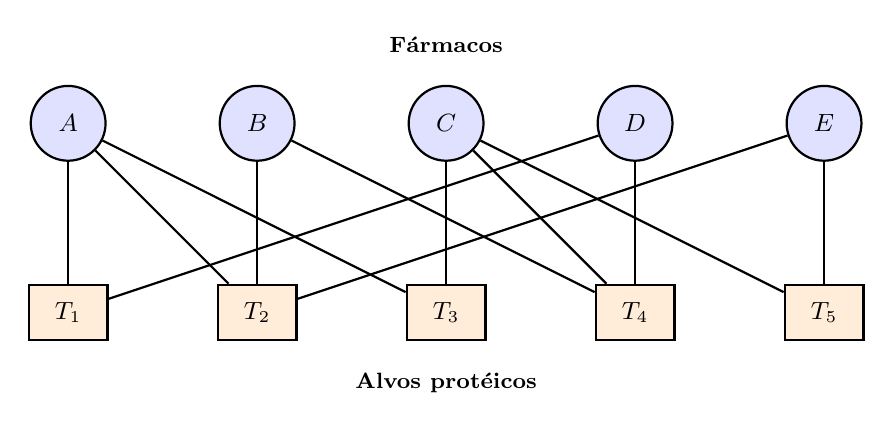
\begin{tikzpicture}[
  every node/.style={font=\small},
  farmaco/.style={circle, draw=black, thick, fill=blue!12, minimum size=0.95cm, inner sep=1pt},
  alvo/.style={rectangle, draw=black, thick, fill=orange!15, minimum width=1.0cm, minimum height=0.7cm, inner sep=2pt},
  aresta/.style={thick}
]
\node[farmaco] (A) at (0,2.4) {$A$};
\node[farmaco] (B) at (2.4,2.4) {$B$};
\node[farmaco] (C) at (4.8,2.4) {$C$};
\node[farmaco] (D) at (7.2,2.4) {$D$};
\node[farmaco] (E) at (9.6,2.4) {$E$};
\node[alvo] (T1) at (0,0) {$T_1$};
\node[alvo] (T2) at (2.4,0) {$T_2$};
\node[alvo] (T3) at (4.8,0) {$T_3$};
\node[alvo] (T4) at (7.2,0) {$T_4$};
\node[alvo] (T5) at (9.6,0) {$T_5$};
\draw[aresta] (A) -- (T1);
\draw[aresta] (A) -- (T2);
\draw[aresta] (A) -- (T3);
\draw[aresta] (B) -- (T2);
\draw[aresta] (B) -- (T4);
\draw[aresta] (C) -- (T3);
\draw[aresta] (C) -- (T4);
\draw[aresta] (C) -- (T5);
\draw[aresta] (D) -- (T1);
\draw[aresta] (D) -- (T4);
\draw[aresta] (E) -- (T2);
\draw[aresta] (E) -- (T5);
\node[font=\footnotesize] at (4.8,3.4) {\textbf{Fármacos}};
\node[font=\footnotesize] at (4.8,-0.9) {\textbf{Alvos protéicos}};
\end{tikzpicture}
\caption{Grafo bipartido fármaco-alvo usado em farmacologia de redes. Os nós azuis representam fármacos ($A, B, C, D, E$); os nós laranja representam alvos protéicos ($T_1, \ldots, T_5$). Cada aresta denota afinidade significativa reportada em bases como DrugBank, ChEMBL ou BindingDB. A promiscuidade de um fármaco é simplesmente seu grau no grafo: aqui, $A$ e $C$ têm grau 3, $B$, $D$ e $E$ têm grau 2. A sobreposição de alvos --- por exemplo, $T_2$ compartilhado por $A$, $B$ e $E$ --- é o ponto de partida para hipóteses de reposicionamento e de previsão de efeitos adversos compartilhados.}
\label{fig:13-bipartido}
\end{figure}

onde valores altos indicam compostos com perfil farmacológico amplo --- candidatos tanto a reposicionamento quanto a efeitos adversos. Fármacos com promiscuidade muito alta, como muitos psicotrópicos e imunossupressores, tendem a apresentar janelas terapêuticas estreitas justamente porque sua ação distribuída atravessa múltiplas redes.


A farmacocinética --- literalmente, ``o que o corpo faz com o fármaco'' --- é a disciplina que descreve, por meio de modelos matemáticos, a evolução temporal da concentração de um composto no organismo após sua administração. Compreende quatro processos resumidos pelo acrônimo \emph{ADME}: absorção (entrada do composto na corrente sanguínea a partir do sítio de administração), distribuição (dispersão pelos tecidos), metabolismo (biotransformação, predominantemente hepática) e excreção (eliminação, majoritariamente renal). Cada um desses processos é quantificável, e a integração dos quatro fornece a curva de concentração plasmática --- a base sobre a qual regimes posológicos são desenhados. A farmacodinâmica, complementarmente, descreve ``o que o fármaco faz com o corpo'': a relação entre a concentração alcançada e o efeito terapêutico (ou tóxico) observado. Juntas, farmacocinética e farmacodinâmica --- abreviadas PK/PD --- constituem o arcabouço formal que conecta dosagem, exposição e efeito.

A absorção depende crucialmente das propriedades físico-químicas do composto --- solubilidade aquosa, lipofilicidade (medida pelo $\log P$ octanol-água), peso molecular, capacidade de formar ligações de hidrogênio --- e da via de administração. Fármacos administrados por via oral precisam atravessar o epitélio gastrointestinal e, em muitos casos, sobreviver ao metabolismo de primeira passagem no fígado antes de alcançar a circulação sistêmica. A distribuição é modulada pela ligação a proteínas plasmáticas (especialmente albumina), pela permeabilidade das membranas teciduais e pela afinidade por tecidos específicos --- muitos compostos lipofílicos acumulam-se em tecido adiposo, formando um reservatório que prolonga seu tempo de ação. O metabolismo é dominado, em mais de setenta por cento dos fármacos, pela família do citocromo P450 --- um conjunto de isoenzimas hepáticas (CYP3A4, CYP2D6, CYP2C9, CYP2C19, entre outras) que oxidam os compostos para torná-los mais hidrofílicos e excretáveis. As variantes genéticas nessas isoenzimas --- polimorfismos --- são uma fonte central de variabilidade interindividual na resposta a fármacos, e serão tratadas em detalhe na Seção~\ref{sec:13-personalizada}. A excreção, finalmente, combina filtração glomerular, secreção tubular ativa e, em menor grau, eliminação biliar e fecal.

A regra de Lipinski, formulada em 1997 e informalmente conhecida como ``regra dos cinco'', sumariza as propriedades físico-químicas associadas a boa biodisponibilidade oral. Um composto tem alta probabilidade de ser absorvido por via oral se satisfaz, em conjunto, peso molecular inferior a 500~Da, $\log P$ inferior a 5, número de doadores de ligação de hidrogênio igual ou inferior a cinco e número de aceptores igual ou inferior a dez. Embora não seja uma condição necessária nem suficiente --- exceções existem e são bem documentadas --- a regra fornece um filtro heurístico útil nas fases iniciais de desenho, sobretudo para evitar investimentos em compostos cuja estrutura já prenuncia problemas de absorção ou solubilidade. Fármacos que violam uma ou mais dessas propriedades, como é o caso de muitos peptídeos e de alguns antibióticos macrolídeos, são tipicamente administrados por outras vias (intravenosa, inalatória, intramuscular).

A tradução matemática desses processos em modelos tratáveis é o objeto da modelagem PK compartimental. No modelo de um compartimento, o organismo é representado como um único volume $V_d$ (volume de distribuição) no qual o fármaco se distribui instantânea e uniformemente, sendo removido por uma reação de primeira ordem com constante $k_e$. A equação diferencial ordinária que governa a concentração $C(t)$ após uma dose intravenosa em bolus é
\begin{equation*}
\frac{\mathrm{d}C}{\mathrm{d}t} = -k_e \, C(t),
\end{equation*}
cuja solução, com condição inicial $C(0) = C_0 = \mathrm{Dose}/V_d$, é a exponencial decrescente
\begin{equation*}
C(t) = C_0 \, e^{-k_e t}.
\end{equation*}
Dessa solução derivam diretamente os parâmetros PK fundamentais: a meia-vida de eliminação $t_{1/2} = \ln 2 / k_e$, o clearance $\mathrm{CL} = k_e V_d$ e a área sob a curva $\mathrm{AUC} = C_0 / k_e = \mathrm{Dose}/\mathrm{CL}$. A interpretação clínica é imediata: $t_{1/2}$ informa o intervalo entre doses necessário para manter concentrações terapêuticas, $\mathrm{CL}$ quantifica a capacidade do organismo de eliminar o fármaco e $\mathrm{AUC}$ mede a exposição sistêmica total ao composto. O modelo de um compartimento é uma aproximação razoável para fármacos que se distribuem rapidamente e de modo homogêneo --- a maioria dos compostos hidrofílicos de pequeno porte ---, mas falha para moléculas que se acumulam em tecidos específicos ou apresentam cinética bifásica.

O modelo de dois compartimentos generaliza essa representação introduzindo um compartimento periférico, separado do central por uma membrana de difusão. O compartimento central --- tipicamente plasma e tecidos altamente perfundidos --- recebe a dose inicial e troca fármaco com o periférico --- usualmente gordura, músculo ou outros tecidos de captação mais lenta --- por meio de constantes de transferência $k_{12}$ (central para periférico) e $k_{21}$ (periférico para central). A eliminação ocorre exclusivamente a partir do compartimento central, com constante $k_e$. O sistema de equações diferenciais resultante é
\begin{align*}
\frac{\mathrm{d}C_1}{\mathrm{d}t} &= -(k_e + k_{12}) \, C_1(t) + k_{21} \, C_2(t), \\
\frac{\mathrm{d}C_2}{\mathrm{d}t} &= k_{12} \, C_1(t) - k_{21} \, C_2(t),
\end{align*}
onde $C_1$ e $C_2$ são as concentrações nos compartimentos central e periférico. A solução desse sistema linear é uma soma de duas exponenciais com constantes de tempo distintas --- uma rápida, dominada pela distribuição inicial, e uma lenta, dominada pela eliminação. Essa cinética bifásica é observável experimentalmente em curvas de concentração plasmática de compostos como a lidocaína e o propranolol, e seu reconhecimento é essencial para regimes de dose que pretendam manter concentrações estáveis durante infusões prolongadas. Modelos com três ou mais compartimentos são necessários para fármacos com distribuição tecidual altamente heterogênea --- agentes anestésicos, por exemplo, requerem tipicamente modelos de três compartimentos para descrever suas fases de distribuição e acúmulo em tecido adiposo. A Figura~\ref{fig:13-pk} ilustra esquematicamente os dois modelos canônicos: o de um compartimento, com cinética monoexponencial governada por uma única constante de eliminação $k_e$, e o de dois compartimentos, com cinética biexponencial em que a fase rápida reflete distribuição e a fase lenta reflete eliminação terminal.

\begin{figure}[ht]
\centering
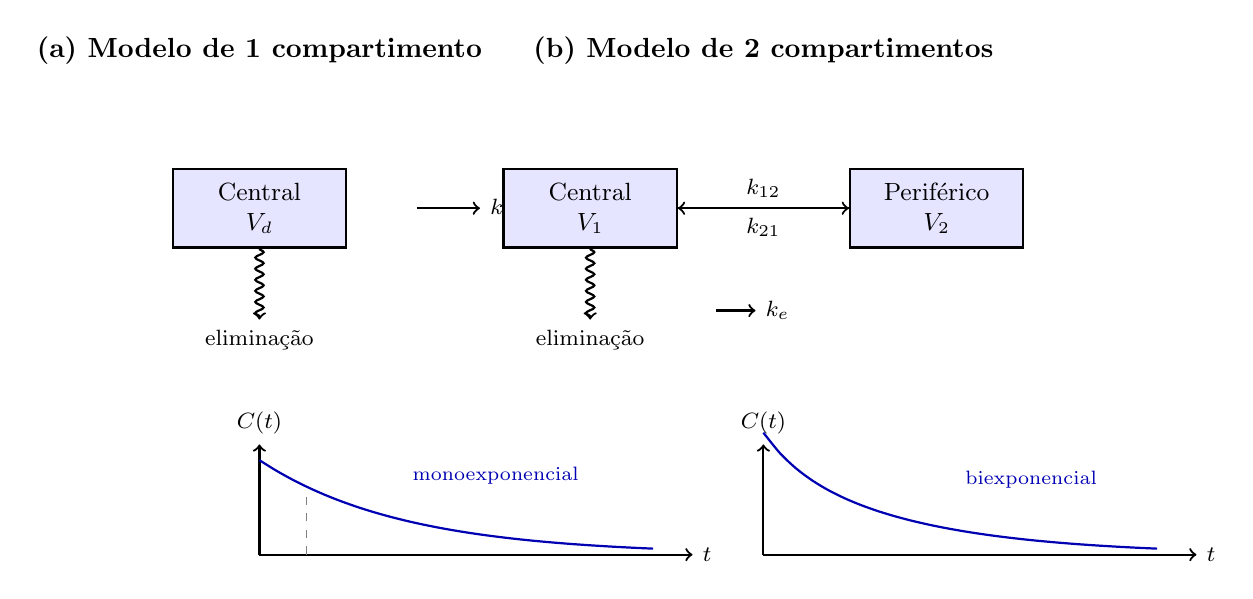
\begin{tikzpicture}[
  every node/.style={font=\small},
  comp/.style={rectangle, draw=black, thick, minimum width=2.2cm, minimum height=1.0cm, fill=blue!10, align=center},
  seta/.style={->, thick}
]
% Painel esquerdo: 1 compartimento
\node[font=\bfseries] at (-3.2, 3.0) {(a) Modelo de 1 compartimento};
\node[comp] (C1) at (-3.2, 1.0) {Central\\$V_d$};
\draw[seta] (-1.2, 1.0) -- ++(0.8, 0) node[right, font=\footnotesize] {$k_e$};
\draw[->, thick, decorate, decoration={snake, amplitude=1.5pt, segment length=4pt}] (C1.south) -- ++(0, -0.9) node[below, font=\footnotesize] {eliminação};
% Painel direito: 2 compartimentos
\node[font=\bfseries] at (3.2, 3.0) {(b) Modelo de 2 compartimentos};
\node[comp] (C2) at (1.0, 1.0) {Central\\$V_1$};
\node[comp] (P2) at (5.4, 1.0) {Periférico\\$V_2$};
\draw[seta] (C2.east) -- node[above, font=\footnotesize] {$k_{12}$} (P2.west);
\draw[seta] (P2.west) -- node[below, font=\footnotesize] {$k_{21}$} (C2.east);
\draw[seta] (2.6, -0.3) -- ++(0.5, 0) node[right, font=\footnotesize] {$k_e$};
\draw[->, thick, decorate, decoration={snake, amplitude=1.5pt, segment length=4pt}] (C2.south) -- ++(0, -0.9) node[below, font=\footnotesize] {eliminação};
% Curva de concentração (esquemática) embaixo de ambos
\begin{scope}[yshift=-3.4cm, xshift=-3.2cm]
  \draw[->, thick] (0,0) -- (5.5, 0) node[right, font=\footnotesize] {$t$};
  \draw[->, thick] (0,0) -- (0, 1.4) node[above, font=\footnotesize] {$C(t)$};
  \draw[domain=0:5, smooth, variable=\x, blue!70!black, thick] plot ({\x}, {1.2*exp(-0.55*\x)});
  \draw[dashed, gray] (0.6, 0) -- (0.6, 0.8);
  \node[font=\scriptsize, blue!70!black] at (3.0, 1.0) {monoexponencial};
\end{scope}
\begin{scope}[yshift=-3.4cm, xshift=3.2cm]
  \draw[->, thick] (0,0) -- (5.5, 0) node[right, font=\footnotesize] {$t$};
  \draw[->, thick] (0,0) -- (0, 1.4) node[above, font=\footnotesize] {$C(t)$};
  \draw[domain=0:5, smooth, variable=\x, blue!70!black, thick] plot ({\x}, {1.2*exp(-0.55*\x) + 0.35*exp(-2.2*\x)});
  \node[font=\scriptsize, blue!70!black] at (3.4, 0.95) {biexponencial};
\end{scope}
\end{tikzpicture}
\caption{Modelos farmacocinéticos compartimentais. (a) Modelo de um compartimento: o organismo é representado por um único volume $V_d$ onde o fármaco se distribui instantaneamente; a eliminação ocorre por uma reação de primeira ordem com constante $k_e$, gerando uma curva de concentração plasmática monoexponencial. (b) Modelo de dois compartimentos: distingue-se um compartimento central (sangue e tecidos altamente perfundidos, volume $V_1$) e um compartimento periférico (tecidos de captação mais lenta, volume $V_2$), conectados por constantes de transferência $k_{12}$ e $k_{21}$; a curva de concentração plasmática resultante é biexponencial, com uma fase rápida dominada pela distribuição e uma fase lenta dominada pela eliminação terminal.}
\label{fig:13-pk}
\end{figure}


A interpretação clínica dos modelos PK passa pela quantificação de seis parâmetros canônicos, cada um deles associado a uma decisão terapêutica específica. O primeiro é $C_{\max}$, a concentração plasmática máxima alcançada após a administração --- determinada pela dose, pela velocidade de absorção e pelo volume de distribuição ---, cujo valor é comparado à janela terapêutica do composto: concentrações abaixo do limite inferior são ineficazes; concentrações acima do limite superior provocam toxicidade. O segundo é $T_{\max}$, o tempo transcorrido até que $C_{\max}$ seja atingido --- informação relevante para fármacos cujo efeito deve ser rápido (analgésicos, por exemplo) ou para os quais se deseja retardar a absorção (formulações de liberação prolongada). O terceiro é $\mathrm{AUC}$, a área sob a curva de concentração em função do tempo --- integral que mede a exposição total do organismo ao fármaco e é proporcional à dose administrada dividida pelo clearance. O quarto é $t_{1/2}$, a meia-vida de eliminação --- intervalo de tempo após o qual a concentração plasmática cai a metade de seu valor ---, que determina o intervalo entre doses em regime de administração repetida: tipicamente, três a cinco meias-vidas são necessárias para atingir o estado de equilíbrio. O quinto é $V_d$, o volume de distribuição aparente --- volume teórico necessário para que a dose administrada produza a concentração observada ---, que pode exceder o volume corporal real para fármacos que se acumulam extensivamente em tecidos (indicando $V_d$ da ordem de centenas a milhares de litros). O sexto é $\mathrm{CL}$, o clearance --- volume de plasma completamente depurado do fármaco por unidade de tempo ---, que mede a capacidade global de eliminação do organismo e, em conjunto com a dose, determina $\mathrm{AUC}$.

A relação entre esses seis parâmetros e a equação do modelo de um compartimento é imediata. Para uma dose intravenosa em bolus, $\mathrm{AUC} = C_0/k_e = \mathrm{Dose}/\mathrm{CL}$, o que permite calcular o clearance diretamente a partir de medidas experimentais de $\mathrm{AUC}$: $\mathrm{CL} = \mathrm{Dose}/\mathrm{AUC}$. O estado de equilíbrio em administração repetida é atingido quando a taxa de administração iguala a taxa de eliminação, e a concentração média no equilíbrio é $\bar{C} = \mathrm{AUC}_{\tau}/\tau$, onde $\tau$ é o intervalo entre doses e $\mathrm{AUC}_{\tau}$ é a área sob a curva em um único intervalo. Em regimes de infusão contínua, a concentração no equilíbrio é simplesmente $\bar{C} = R/\mathrm{CL}$, onde $R$ é a taxa de infusão (dose por unidade de tempo). Essas relações, embora elementares, são a base sobre a qual toda a farmacologia clínica de dose-múltipla se sustenta --- e ilustram como um modelo matemático simples (um único compartimento, primeira ordem) pode orientar decisões terapêuticas complexas.

A biologia de sistemas adiciona uma camada de sofisticação ao PK/PD tradicional por meio da integração de modelos mecanísticos com dados multi-ômicos. Em vez de tratar o organismo como uma caixa-preta cujas constantes PK ($k_e$, $V_d$, $k_{12}$, $k_{21}$) são ajustadas empiricamente a partir de curvas experimentais, modelos contemporâneos buscam explicar essas constantes em termos de propriedades moleculares: expressão tecidual de transportadores de influxo e efluxo, abundância de isoenzimas do citocromo P450, polimorfismos genéticos que afetam a atividade enzimática, presença de patologias que alteram a função hepática ou renal. O resultado é o que se convencionou chamar de \emph{modelo PBPK} (\emph{physiologically-based pharmacokinetic model}), no qual cada tecido é representado como um compartimento separado com fluxos sanguíneos e permeabilidades específicas, e os parâmetros do modelo são estimados a partir de dados pré-clínicos e clínicos de modo fisicamente interpretável. Embora mais complexo que o modelo de um ou dois compartimentos, o PBPK permite prever concentrações teciduais em populações específicas --- pediátricas, geriátricas, com insuficiência renal --- que não foram diretamente estudadas em ensaios clínicos, e por essa razão tem sido cada vez mais adotado tanto na indústria farmacêutica quanto em agências reguladoras como a FDA e a EMA.

A modelagem PK/PD computacional tornou-se acessível com pacotes de software de uso geral. Em Python, a integração numérica de sistemas de equações diferenciais é imediata por meio da função \texttt{odeint} do \texttt{SciPy}, e a comparação entre soluções analíticas e numéricas fornece um exercício pedagógico valioso para internalizar o comportamento temporal dos compostos. A Seção~\ref{sec:13-exercicios} apresenta um exercício guiado no qual o leitor implementa o modelo de um compartimento, simula a concentração plasmática ao longo de vinte e quatro horas, e compara a meia-vida estimada com o valor analítico. Exercícios adicionais estendem a análise ao modelo de dois compartimentos e à estimativa de parâmetros por ajuste a dados experimentais sintéticos.


A integração da biologia de sistemas com o desenvolvimento clínico de fármacos transforma a maneira como ensaios clínicos são concebidos, conduzidos e interpretados. As quatro fases tradicionais mantêm sua estrutura --- a fase I avalia segurança e farmacocinética em voluntários saudáveis (vinte a cem participantes), a fase II avalia eficácia preliminar e dose em pacientes com a doença-alvo (cem a quinhentos), a fase III confirma eficácia em larga escala e monitora efeitos adversos (mil a cinco mil pacientes), e a fase IV conduz vigilância pós-comercialização ---, mas cada uma delas incorpora crescentemente marcadores moleculares que estratificam pacientes, preveem resposta e antecipam toxicidade. Essa estratificação tem implicações estatísticas profundas: um ensaio enriquecido com respondedores previstos pode detectar o mesmo efeito terapêutico com uma fração dos pacientes necessários em um ensaio não estratificado, acelerando cronogramas e reduzindo custos. Simultaneamente, levanta questões éticas e regulatórias sobre o que constitui evidência suficiente para restringir a indicação de um fármaco a um subgrupo molecular específico, em vez de estendê-lo à população geral.

Os \emph{adaptive trials} --- ensaios cujo desenho é modificado em resposta a dados intermediários --- constituem outra contribuição metodológica relevante. Em um esquema adaptativo, a alocação de pacientes entre braços de tratamento pode ser ajustada dinamicamente para favorecer o braço com resposta superior, os critérios de inclusão podem ser refinados com base em biomarcadores identificados nos primeiros pacientes, e mesmo o número total de participantes pode ser recalculado à medida que evidências acumulam. Esses desenhos, formalmente introduzidos por Bauer e colegas no início dos anos 2000 e adotados em escala crescente pela indústria farmacêutica e por agências reguladoras, representam uma aplicação direta de princípios de controle bayesiano e otimização sequencial --- e só se tornaram computacionalmente viáveis com o poder de processamento disponível nas últimas duas décadas. Ensaios clínicos em oncologia, onde a heterogeneidade molecular é extrema, são candidatos naturais a desenhos adaptativos, e diversos fármacos aprovados nos últimos anos --- vemurafenibe, olaparibe, osimertinibe --- devem parte de seu sucesso regulatório a ensaios com componentes adaptativos.

O conceito de \emph{digital twin} --- réplica computacional personalizada de um paciente individual --- sintetiza várias das ideias introduzidas neste capítulo. Um digital twin integra dados genômicos, transcriptômicos, proteômicos, metabólomicos, de imagem e clínicos de um paciente específico em um modelo computacional capaz de simular a progressão da doença e a resposta a intervenções terapêuticas antes que essas intervenções sejam administradas. Em sua forma mais ambiciosa, o digital twin incorpora um modelo PBPK com parâmetros individuais, um modelo de redes regulatórias estimado a partir do transcriptoma do paciente, e um modelo de evolução tumoral (no caso de câncer) calibrado por meio de biópsias líquidas seriadas. A simulação resultante permite comparar, in silico, a eficácia prevista de diferentes protocolos terapêuticos e identificar, também in silico, regimes de dose personalizados que maximizem a probabilidade de resposta e minimizem o risco de toxicidade.

A implementação prática de digital twins esbarra, ainda, em desafios técnicos e regulatórios consideráveis. A integração de dados multi-ômicos heterogêneos em um modelo coerente exige pipelines computacionais robustos e reprodutíveis --- tema central do Capítulo~\ref{cap:11}. A estimativa de parâmetros individuais a partir de dados esparsos é um problema estatístico de alta dimensionalidade, no qual o número de parâmetros do modelo excede tipicamente o número de observações disponíveis para um único paciente, exigindo métodos de regularização e priors informativos derivados de populações. A validação prospectiva --- comparar previsões do digital twin com desfechos clínicos reais --- ainda é limitada a poucos estudos-piloto, e a aceitação regulatória desses modelos como evidência suficiente para decisões terapêuticas permanece em construção. Não obstante, investimentos significativos de grandes empresas farmacêuticas, de empresas de tecnologia e de programas de pesquisa acadêmica --- notadamente o projeto \emph{Living Biobank} da Universidade de Harvard e o consórcio \emph{Virtual Physiological Human} da Comissão Europeia --- indicam que o conceito deixará progressivamente o domínio da demonstração técnica para ocupar uma posição central na prática clínica da próxima década. A Seção~\ref{sec:13-aplicacoes} deste capítulo apresenta estudos de caso concretos em que princípios da biologia de sistemas já se traduzem em terapias aprovadas e em decisões clínicas padronizadas.


\section{Doenças Complexas}
\label{sec:13-doencas}

As doenças tratadas neste capítulo --- câncer, doenças cardiovasculares, diabetes, doenças neurodegenerativas --- têm em comum uma característica que as distingue das doenças mendelianas clássicas e que torna a abordagem reducionista tradicional insuficiente: elas são \emph{doenças de redes}, não de genes isolados. Cada uma delas emerge da combinação de múltiplas variantes genéticas, frequentemente com penetrância baixa e efeito aditivo; de alterações epigenéticas, transcriptômicas e proteômicas; de fatores ambientais e de estilo de vida que modulam a expressão gênica e a função celular; e de alterações sistêmicas --- inflamação crônica de baixo grau, disfunção metabólica, remodelamento do microambiente --- que afetam simultaneamente múltiplos órgãos e tecidos. A consequência prática dessa complexidade é que nenhum marcador isolado --- um único SNP, um único nível sérico de uma proteína, uma única medida clínica --- captura adequadamente o estado do paciente ou o risco de progressão. A caracterização molecular de uma doença complexa exige, por conseguinte, perfis multi-ômicos --- genômica, transcriptômica, proteômica, metabolômica, metagenômica --- analisados em conjunto e interpretados à luz da topologia das redes biológicas relevantes.

O câncer é o exemplo paradigmático dessa transição conceitual. A visão tradicional --- um gene, uma mutação, uma doença --- foi durante décadas o motor da oncologia molecular: a descoberta dos oncogenes nos anos 1970 e 1980 (RAS, MYC, EGFR, entre outros) e dos genes supressores tumorais (TP53, RB1, PTEN) estabeleceu que mutações específicas em genes específicos podiam causar transformação celular. Essa visão foi, e continua sendo, correta no nível molecular --- é verdade que mutações em RAS ativam constitutivamente a via MAPK/ERK, que mutações em TP53 abolitam a resposta a danos no DNA, que amplificação de MYC eleva a taxa de transcrição gênica. Mas mostrou-se insuficiente para explicar o comportamento clínico dos tumores: por que dois pacientes com a mesma mutação em EGFR têm respostas diferentes ao gefitinibe; por que um mesmo tumor pode regredir com uma droga e recrescer com uma mutação de resistência; por que metástases derivadas do mesmo tumor primário apresentam perfis moleculares distintos. A resposta, hoje consensual, é que o câncer é uma doença de redes regulatórias alteradas, na qual o fenótipo maligno --- proliferação descontrolada, evasão de apoptose, angiogênese, metástase --- emerge da interação de dezenas a centenas de alterações moleculares operando em módulos funcionais interconectados.

Hanahan e Weinberg, em sua revisão seminal de 2000 na \emph{Cell} e em sua atualização de 2011, organizaram esse conhecimento em uma lista de \emph{hallmarks} --- capacidades celulares adquiridas durante o desenvolvimento tumoral --- que se tornou referência para a oncologia moderna. As seis características originais eram: sinalização proliferativa sustentada, evasão de supressores de crescimento, resistência à morte celular, imortalidade replicativa, angiogênese induzida e capacidade de invasão e metástase. A revisão de 2011 adicionou duas características emergentes --- reprogramação metabólica e evasão da resposta imune --- e duas características facilitadoras --- instabilidade genômica e mutação, e inflamação promotora de tumor. Cada hallmark corresponde a alterações moleculares específicas em redes bem caracterizadas: a sinalização proliferativa sustentada envolve as vias RAS/MAPK, PI3K/AKT e JAK/STAT; a evasão apoptótica envolve a família BCL-2, a via do TP53 e a sinalização de morte celular programada; a reprogramação metabólica envolve o efeito Warburg, a glutaminólise e a síntese lipídica; e assim por diante. O ponto crucial é que essas redes estão interligadas, formando uma \emph{rede oncogênica integrada} cuja topologia determina tanto o fenótipo tumoral quanto a vulnerabilidade terapêutica. A Figura~\ref{fig:13-hallmarks} organiza os dez hallmarks em torno da célula tumoral e dos módulos moleculares que os sustentam.

\begin{figure}[ht]
\centering
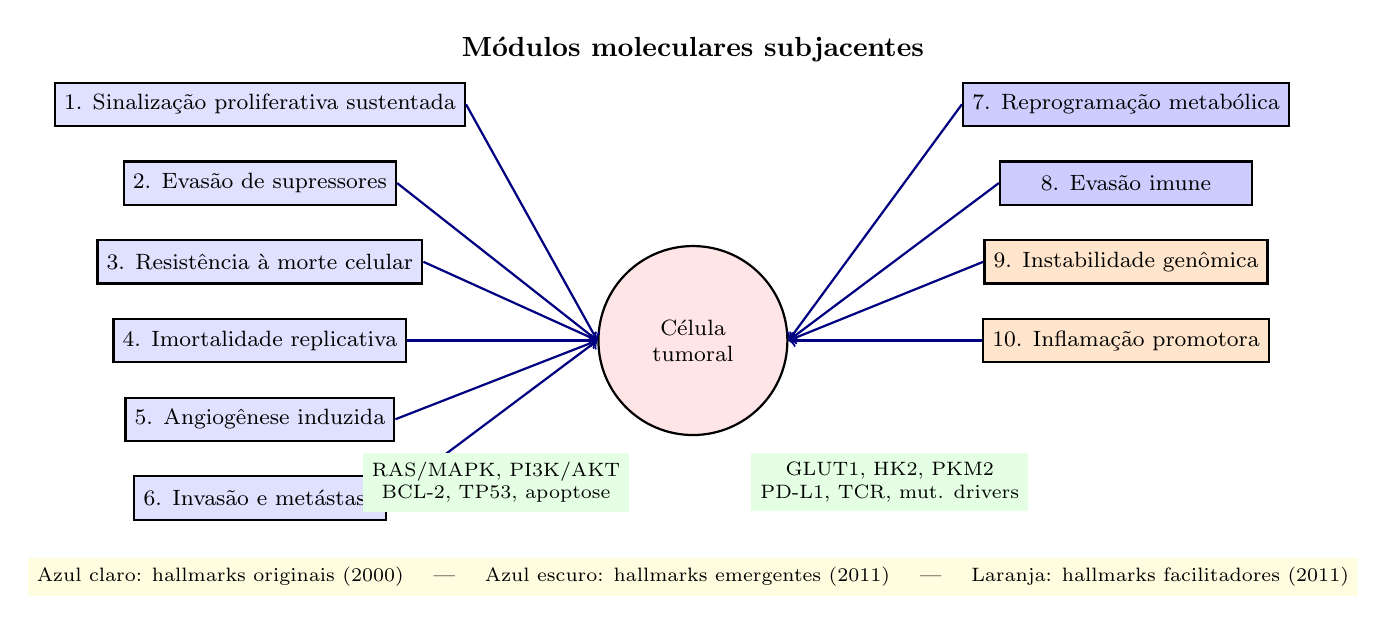
\begin{tikzpicture}[
  every node/.style={font=\footnotesize, align=center},
  cell/.style={circle, draw=black, thick, fill=red!10, minimum size=2.4cm, inner sep=2pt},
  hall/.style={rectangle, draw=black, thick, minimum width=3.2cm, minimum height=0.55cm, fill=blue!12},
  leg/.style={font=\scriptsize, align=center, fill=yellow!12}
]
% Célula tumoral central
\node[cell] (C) at (0, 0) {Célula\\tumoral};

% Hallmarks originais (2000) - 6
\node[hall] (h1) at (-5.5, 3.0) {1. Sinalização proliferativa sustentada};
\node[hall] (h2) at (-5.5, 2.0) {2. Evasão de supressores};
\node[hall] (h3) at (-5.5, 1.0) {3. Resistência à morte celular};
\node[hall] (h4) at (-5.5, 0.0) {4. Imortalidade replicativa};
\node[hall] (h5) at (-5.5, -1.0) {5. Angiogênese induzida};
\node[hall] (h6) at (-5.5, -2.0) {6. Invasão e metástase};

% Hallmarks adicionados (2011) - 4
\node[hall, fill=blue!20] (h7) at (5.5, 3.0) {7. Reprogramação metabólica};
\node[hall, fill=blue!20] (h8) at (5.5, 2.0) {8. Evasão imune};
\node[hall, fill=orange!20] (h9) at (5.5, 1.0) {9. Instabilidade genômica};
\node[hall, fill=orange!20] (h10) at (5.5, 0.0) {10. Inflamação promotora};

% Conexões
\foreach \n in {1,2,3,4,5,6} {
  \draw[->, thick, blue!50!black] (h\n.east) -- (C.west);
}
\foreach \n in {7,8,9,10} {
  \draw[->, thick, blue!50!black] (h\n.west) -- (C.east);
}

% Legenda
\node[leg] at (0, -3.0) {Azul claro: hallmarks originais (2000) \quad | \quad Azul escuro: hallmarks emergentes (2011) \quad | \quad Laranja: hallmarks facilitadores (2011)};

% Módulos moleculares
\node[font=\bfseries] at (0, 3.7) {Módulos moleculares subjacentes};
\node[font=\scriptsize, align=center, fill=green!10] at (-2.5, -1.8) {RAS/MAPK, PI3K/AKT\\BCL-2, TP53, apoptose};
\node[font=\scriptsize, align=center, fill=green!10] at (2.5, -1.8) {GLUT1, HK2, PKM2\\PD-L1, TCR, mut. drivers};
\end{tikzpicture}
\caption{Os dez hallmarks do câncer segundo Hanahan e Weinberg (2000, atualizado em 2011), organizados em torno da célula tumoral. Os seis hallmarks originais --- sinalização proliferativa sustentada, evasão de supressores, resistência à morte celular, imortalidade replicativa, angiogênese e metástase --- correspondem a propriedades celulares adquiridas durante a tumorigênese. A atualização de 2011 adicionou a reprogramação metabólica e a evasão imune (hallmarks emergentes), além de instabilidade genômica e inflamação promotora (hallmarks facilitadores). Os módulos moleculares subjacentes --- vias de sinalização, efetores apoptóticos, transportadores metabólicos, checkpoints imunes --- formam a \emph{rede oncogênica integrada} cuja topologia determina o fenótipo e a vulnerabilidade terapêutica do tumor.}
\label{fig:13-hallmarks}
\end{figure}

O efeito Warburg --- a observação, feita por Otto Warburg nos anos 1920, de que células tumorais apresentam glicólise aeróbica preferencial em detrimento da fosforilação oxidativa --- é, ao mesmo tempo, um exemplo histórico e um caso atual de reprogramação metabólica. A explicação convencional --- de que a glicólise seria consequência de dano mitocondrial --- mostrou-se incompleta: muitas células tumorais têm mitocôndrias funcionais e ainda assim preferem glicólise. A interpretação sistêmica reconhece que a glicólise aeróbica oferece vantagens específicas para a célula tumoral em proliferação: gera ATP mais rapidamente, embora em menor rendimento por molécula de glicose; produz intermediários biossintéticos (ribose para nucleotídeos, acetil-CoA para lipídios, aminoácidos não-essenciais) que alimentam a síntese de biomassa necessária à divisão celular; e acidifica o microambiente extracelular, favorecendo invasão e supressão imune. As alterações moleculares que sustentam esse fenótipo incluem superexpressão do transportador de glicose GLUT1, das isoenzimas glicolíticas HK2 e PKM2, e de enzimas da via da glutaminólise --- alvos terapêuticos potenciais, com inibidores em desenvolvimento clínico.

A heterogeneidade tumoral --- variação entre células de um mesmo tumor, entre tumores de pacientes diferentes, e entre tumor primário e metástases --- é talvez o maior obstáculo à terapia curativa do câncer e a área em que a biologia de sistemas tem mais a contribuir. A heterogeneidade intratumoral --- a coexistência, em um mesmo tumor, de subpopulações celulares com perfis genômicos e transcriptômicos distintos --- emerge de dois processos complementares: a instabilidade genômica das células tumorais, que gera continuamente variantes alélicas novas, e a seleção darwiniana local, que expande os clones mais aptos em cada nicho do microambiente. Consequências práticas incluem a resistência a terapias de alvo único --- um clone minoritário pré-existente com a mutação de resistência acaba selecionado pelo tratamento --- e a limitação de biópsias isoladas, que podem não capturar a diversidade clonal. A heterogeneidade intertumoral --- a variação entre pacientes com o mesmo diagnóstico histológico --- é a base da medicina personalizada em oncologia: tumores de mama classificados como ``ductais'' pela histologia convencional correspondem a subtipos moleculares distintos (luminal A, luminal B, HER2-enriquecido, basal-símile, normal-símile) com prognósticos e terapêuticas diferentes, como será detalhado na Seção~\ref{sec:13-personalizada}.


As doenças cardiovasculares oferecem um segundo exemplo paradigmático de doença sistêmica, com uma camada adicional de complexidade representada por sua estreita interação com fatores ambientais e comportamentais. A aterosclerose, lesão patológica central do infarto do miocárdio e do acidente vascular cerebral, não é mais vista como simples acúmulo de lipídios na parede arterial --- a ``hipótese lipídica'' dos anos 1960 ---, mas como um processo inflamatório crônico no qual a retenção subendotelial de LDL oxidado desencadeia recrutamento de monócitos, diferenciação em macrófagos, formação de células espumosas (\emph{foam cells}) e secreção de citocinas que sustentam a inflamação local. Sobre essa base inflamatória, a progressão da placa depende de migração e proliferação de células musculares lisas, de angiogênese intraplaca, de apoptose de células espumosas com formação de núcleo necrótico, e finalmente de ruptura da cápsula fibrosa --- evento que expõe material trombogênico à corrente sanguínea e desencadeia trombose aguda. Cada um desses passos é mediado por redes moleculares específicas: as LDL oxidadas sinalizam via receptores \emph{scavenger} (SR-A, CD36, LOX-1) e via receptores Toll-like (TLR4); a inflamação depende das vias NF-\emph{k}B e das citocinas IL-1$\beta$, IL-6 e TNF; a trombose envolve a cascata de coagulação e a ativação plaquetária.

A biologia de sistemas oferece à cardiologia duas ferramentas conceituais particularmente férteis: o conceito de \emph{módulo de risco} e o \emph{score de risco poligênico}. O primeiro identifica subconjuntos de genes, proteínas ou metabólitos cujas alterações correlacionam-se com risco cardiovascular de modo mais robusto que qualquer marcador isolado --- é o que se observa, por exemplo, em painéis de biomarcadores que combinam troponina de alta sensibilidade, NT-proBNP, PCR ultrasensível e razão triglicerídeos/HDL, fornecendo predição de eventos que supera a dos fatores de risco tradicionais considerados individualmente. O segundo --- construído a partir de estudos de associação genômica ampla (GWAS) em centenas de milhares de indivíduos --- integra o efeito de centenas a milhares de variantes comuns, cada uma com penetrância muito baixa, em um único número que estima a predisposição genética do indivíduo. Scores poligênicos cardiovasculares estão hoje em fase de implementação clínica prospectiva em vários centros, com resultados iniciais sugerindo utilidade para estratificação de pacientes em risco intermediário, onde os algoritmos clássicos baseados apenas em fatores clínicos têm baixo poder discriminante.

O diabetes mellitus tipo 2 ilustra uma doença na qual a integração multi-órgão é literalmente a regra fisiopatológica. A hiperglicemia crônica --- traço definidor da doença --- emerge da combinação de resistência à insulina nos tecidos periféricos (músculo esquelético, fígado, tecido adiposo) e disfunção das células $\beta$ pancreáticas, que perdem progressivamente a capacidade de secretar insulina em resposta à glicose. Mas a doença não se reduz a essa díade: a resistência à insulina está estreitamente ligada à obesidade visceral e à inflamação do tecido adiposo, que libera ácidos graxos livres, adipocinas inflamatórias (TNF, IL-6, resistina) e reduz a secreção de adiponectina protetora. O músculo esquelético, em resistência insulínica, apresenta captação reduzida de glicose e acúmulo intracelular de lipídios, formando diacilgliceróis e ceramidas que interferem com a sinalização do receptor de insulina. O fígado, em esteatose hepática não alcoólica, aumenta a produção endógena de glicose via gliconeogênese e libera VLDL em excesso, contribuindo para a dislipidemia aterogênica. E a hiperglicemia crônica, por sua vez, danifica o endotélio (glicação de proteínas, estresse oxidativo, via dos polióis), o glomérculo renal (nefropatia diabética), a retina (retinopatia) e os nervos periféricos (neuropatia), gerando as complicações crônicas que dominam o prognóstico da doença.

A síndrome metabólica --- denominação clínica que combina obesidade abdominal, hiperglicemia, hipertensão arterial, dislipidemia aterogênica e estado pró-inflamatório --- formaliza o reconhecimento de que esses componentes compartilham mecanismos fisiopatológicos comuns e tendem a coexistir. A biologia de sistemas oferece modelos quantitativos dessa síndrome por meio de modelos de homeostase glicose-insulina (modelo HOMA, que estima resistência insulínica a partir de medidas basais de glicose e insulina) e de modelos integrados multi-órgão que simulam a interação entre pâncreas, fígado, músculo e tecido adiposo em escala temporal de horas a anos. Esses modelos permitem testar in silico o efeito de intervenções --- perda de peso, exercício, metformina, inibidores de SGLT2, agonistas de GLP-1 --- sobre trajetórias de longo prazo da doença, e informam o desenho de estratégias terapêuticas combinadas.

As doenças neurodegenerativas --- doença de Alzheimer, doença de Parkinson, esclerose lateral amiotrófica, Huntington --- representam o terceiro grupo de doenças complexas abordado neste capítulo. Comum a todas elas é uma cascata patológica multifatorial --- envolvendo acúmulo de proteínas mal enoveladas, disfunção mitocondrial, estresse oxidativo, neuroinflamação e, eventualmente, morte neuronal --- que progride ao longo de anos a décadas. Na doença de Alzheimer, duas lesões histopatológicas dominam: as placas extracelulares de peptídeo $\beta$-amiloide, geradas por clivagem anômala da proteína precursora amiloide (APP) pelas secretases $\beta$ e $\gamma$, e os emaranhados neurofibrilares intracelulares de proteína tau hiperfosforilada. A essas lesões somam-se perda sináptica precoce, neuroinflamação mediada por micróglia e astrócitos, disfunção mitocondrial e estresse oxidativo --- componentes que, em conjunto, determinam o declínio cognitivo progressivo. A doença de Parkinson, por outro lado, caracteriza-se pela perda de neurônios dopaminérgicos da substância negra pars compacta e pela presença de corpos de Lewy --- inclusões intracelulares compostas principalmente de $\alpha$-sinucleína agregada.

A análise de redes aplicada às doenças neurodegenerativas identifica módulos de doença distintos --- módulo de processamento de $\beta$-amiloide, módulo de fosforilação de tau, módulo de autofagia, módulo de resposta inflamatória --- cujas perturbações convergem sobre o fenótipo clínico comum. Essa decomposição modular é importante por duas razões. Primeiro, explica por que fármacos desenhados contra um único componente (anti-amiloide, por exemplo) frequentemente falham em ensaios clínicos: o módulo amiloide é apenas um dos vários alterados, e sua modulação isolada não é suficiente para reverter a cascata. Segundo, sugere alvos terapêuticos combinados ou estratégias que atuem sobre mecanismos compartilhados por múltiplos módulos --- como restauração da função autofágica, redução da neuroinflamação crônica, ou melhora da função mitocondrial. A farmacologia de redes, nesse contexto, deixa de ser abstração metodológica e torna-se estratégia terapêutica concreta para doenças em que décadas de tentativas reducionistas produziram resultados decepcionantes.


O conceito de \emph{módulo de doença}, formalizado por Menche e colaboradores em artigo de 2015 na \emph{Science}, sintetiza em uma definição operacional a intuição central da medicina de redes: uma doença corresponde a um conjunto de componentes moleculares --- genes, proteínas, metabólitos --- que estão topologicamente próximos no interactoma humano e cujas perturbações, em conjunto, produzem um fenótipo patológico reconhecível. Mais precisamente, um módulo de doença é definido como uma ``bola'' (\emph{ball}) no grafo do interactoma centrada em um conjunto de genes associados à doença: o conjunto inclui os próprios genes de doença e seus vizinhos diretos no grafo, e o módulo é delimitado por um raio topológico que maximiza a separação entre proteínas de doença e proteínas aleatoriamente amostradas. A análise sistemática de módulos de doença em centenas de fenótipos catalogados em bases como o OMIM (\emph{Online Mendelian Inheritance in Man}) e o GWAS Catalog revelou três propriedades fundamentais. Primeiro, módulos de doenças distintas tendem a ocupar regiões topologicamente distintas do interactoma, refletindo a especificidade mecanística de cada patologia. Segundo, módulos de doenças clinicamente relacionadas --- por exemplo, doenças autoimunes, ou doenças metabólicas, ou diferentes tipos de câncer --- apresentam sobreposição substancial, refletindo mecanismos patogênicos compartilhados. Terceiro, e talvez mais relevante do ponto de vista clínico, a sobreposição entre módulos de doenças clinicamente não relacionadas explica \emph{comorbidades} --- a coexistência em um mesmo paciente de duas ou mais doenças cuja associação não seria esperada a partir dos respectivos fatores de risco conhecidos. A Figura~\ref{fig:13-modulo} ilustra esquematicamente essa construção: o módulo de cada doença é uma ``bola'' (ball) no interactoma centrada em seus genes associados, e a sobreposição entre bolas representa a base mecanística das comorbidades.

\begin{figure}[ht]
\centering
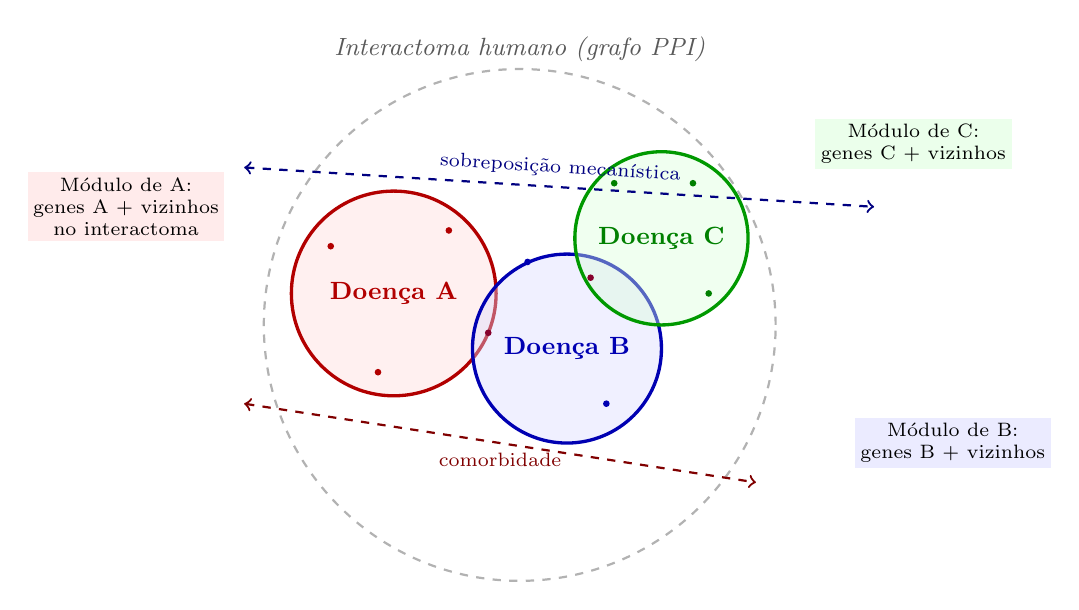
\begin{tikzpicture}[
  every node/.style={font=\small, align=center},
  interatoma/.style={circle, draw=gray!60, thick, dashed, minimum size=6.5cm},
  modA/.style={circle, draw=red!70!black, very thick, fill=red!15, minimum size=2.6cm, fill opacity=0.4},
  modB/.style={circle, draw=blue!70!black, very thick, fill=blue!15, minimum size=2.4cm, fill opacity=0.4},
  modC/.style={circle, draw=green!60!black, very thick, fill=green!15, minimum size=2.2cm, fill opacity=0.4},
  labelA/.style={font=\bfseries\small, red!70!black},
  labelB/.style={font=\bfseries\small, blue!70!black},
  labelC/.style={font=\bfseries\small, green!50!black},
  anotA/.style={font=\scriptsize, align=center, fill=red!8, rectangle, inner sep=2pt},
  anotB/.style={font=\scriptsize, align=center, fill=blue!8, rectangle, inner sep=2pt},
  anotC/.style={font=\scriptsize, align=center, fill=green!8, rectangle, inner sep=2pt}
]
\node[interatoma] (I) at (0,0) {};
\node[font=\itshape\small, gray!70!black] at (0, 3.5) {Interactoma humano (grafo PPI)};
\node[modA] (A) at (-1.6, 0.4) {};
\node[modB] (B) at (0.6, -0.3) {};
\node[modC] (C) at (1.8, 1.1) {};
\node[labelA] at (-1.6, 0.4) {Doença A};
\node[labelB] at (0.6, -0.3) {Doença B};
\node[labelC] at (1.8, 1.1) {Doença C};
% Pontos de genes (decorativos)
\foreach \p in {(-2.4,1.0),(-1.8,-0.6),(-0.9,1.2)} \fill[red!70!black] \p circle (1.2pt);
\foreach \p in {(0.1,0.8),(1.1,-1.0)} \fill[blue!70!black] \p circle (1.2pt);
\foreach \p in {(2.4,0.4),(1.2,1.8),(2.2,1.8)} \fill[green!50!black] \p circle (1.2pt);
\foreach \p in {(0.9,0.6),(-0.4,-0.1)} \fill[purple!70!black] \p circle (1.2pt);
% Anotações
\node[anotA] at (-5.0, 1.5) {Módulo de A:\\genes A + vizinhos\\no interactoma};
\node[anotB] at (5.5, -1.5) {Módulo de B:\\genes B + vizinhos};
\node[anotC] at (5.0, 2.3) {Módulo de C:\\genes C + vizinhos};
% Comorbidades
\draw[<->, thick, red!50!black, dashed] (-3.5, -1.0) -- node[below, font=\scriptsize] {comorbidade} (3.0, -2.0);
\draw[<->, thick, blue!50!black, dashed] (-3.5, 2.0) -- node[above, font=\scriptsize, sloped] {sobreposição mecanística} (4.5, 1.5);
\end{tikzpicture}
\caption{Módulos de doença no interactoma e a base mecanística das comorbidades. Cada doença --- $A$, $B$, $C$ --- corresponde a uma \emph{bola} topológica no grafo do interactoma humano, centrada em seus genes associados e delimitada por um raio que inclui os vizinhos diretos. A sobreposição entre bolas reflete mecanismos moleculares compartilhados --- inflamação crônica, estresse oxidativo, disfunção metabólica --- e é a base mecanística das comorbidades observadas na prática clínica: pares como diabetes tipo 2 e doença cardiovascular, depressão e doença cardiovascular, doença renal crônica e doença cardiovascular, Alzheimer e diabetes tipo 2. A análise sistemática de módulos de doença (Menche et al., 2015) revelou que doenças clinicamente relacionadas ocupam regiões topologicamente próximas do interactoma, e que a sobreposição entre módulos de doenças clinicamente distantes prediz comorbidades antes mesmo de serem observadas epidemiologicamente.}
\label{fig:13-modulo}
\end{figure}

As comorbidades --- definidas como a coexistência em um mesmo paciente de duas doenças em frequência maior do que o esperado pelo acaso --- constituem um dos problemas clínicos mais relevantes da medicina contemporânea, especialmente em populações idosas, e a análise de redes fornece uma explicação sistemática para sua ocorrência. Quando duas doenças --- por exemplo, diabetes tipo 2 e doença cardiovascular aterosclerótica --- compartilham parte de seus módulos moleculares, é porque compartilham vias e mecanismos --- inflamação crônica de baixo grau, estresse oxidativo, disfunção endotelial, alteração do metabolismo lipídico ---, e essa sobreposição mecanística traduz-se, no nível populacional, em taxas de comorbidade acima do esperado. A utilidade clínica dessa observação é dupla: antecipar comorbidades em pacientes recém-diagnosticados e priorizar estratégias terapêuticas que atuem simultaneamente sobre mecanismos compartilhados. O mesmo raciocínio aplica-se a pares como depressão e doença cardiovascular, doença renal crônica e doença cardiovascular, e doença de Alzheimer e diabetes tipo 2 --- todos exemplos bem estabelecidos de comorbidades parcialmente explicadas por sobreposição de módulos.

A classificação de doenças baseada em redes constitui a contrapartida sistêmica da classificação clínica tradicional. A classificação vigente --- codificada na CID (\emph{Classificação Internacional de Doenças}) da OMS e em manuais como o DSM-5 (\emph{Diagnostic and Statistical Manual of Mental Disorders}) --- organiza doenças por órgão, sistema ou sintoma predominante, e tem a vantagem da praticidade e da compatibilidade com séculos de tradição clínica. Tem, no entanto, limitações crescentes à medida que a medicina molecular avança. Dois pacientes com o mesmo diagnóstico clínico --- ``câncer de mama'', ``diabetes tipo 2'', ``asma'' --- podem ter doenças moleculares muito diferentes, com prognósticos e respostas terapêuticas distintas; e dois pacientes com diagnósticos clínicos diferentes podem compartilhar mecanismos moleculares que sugeririam terapias semelhantes. A classificação baseada em redes procura superar essas limitações organizando doenças por seus módulos moleculares, e não por seus sintomas.

Os exemplos concretos de classificação molecular já em uso clínico são múltiplos. No câncer, a classificação molecular de tumores sólidos --- sistematizada em projetos como o \emph{The Cancer Genome Atlas} (TCGA) --- produziu uma taxonomia inteiramente nova, baseada em perfis de expressão gênica, mutações driver e alterações epigenéticas, que já substitui a classificação puramente histológica em diversas decisões terapêuticas. O exemplo mais bem estabelecido é o dos subtipos moleculares de câncer de mama --- luminal A, luminal B, HER2-enriquecido e basal-símile ---, que serão detalhados na Seção~\ref{sec:13-personalizada} por sua importância na medicina personalizada. No diabetes tipo 2, análises recentes identificaram pelo menos cinco subtipos --- um caracterizado por deficiência grave de secreção de insulina, três por graus variados de resistência insulínica, e um por obesidade e idade avançada ---, cada um com perfis de complicações e respostas terapêuticas distintas. Em doenças inflamatórias, a noção de \emph{endotipos} --- subtipos definidos por perfis moleculares de citocinas e células imunes, em vez de apresentação clínica --- está substituindo lentamente a classificação sindrômica clássica. Asma, por exemplo, divide-se em endotipos eosinofílico, neutrofílico e paucigranulocítico, com respostas diferenciadas a corticosteroides e a biológicos como omalizumabe e dupilumabe.

O caminho da classificação molecular à prática clínica é, no entanto, irregular e enfrenta resistência legítima. A classificação clínica tradicional tem a seu favor décadas de observação, validação por desfechos, integração com formação médica e compatibilidade com sistemas de reembolso; substituí-la abruptamente por uma taxonomia molecular --- por mais bem fundamentada --- criaria incertezas práticas. A tendência atual é de coexistência: a classificação clínica permanece como primeira linha de organização, e a estratificação molecular é acrescentada como refinamento secundário para decisões específicas --- escolha terapêutica, prognóstico, aconselhamento genético. Esse modelo híbrido é provavelmente o que permanecerá por décadas, até que a medicina molecular se torne rotineira o suficiente para que a classificação clínica atual pareça tão ultrapassada quanto a classificação dos quatro humores parece hoje.

A integração entre módulos de doença, comorbidades e classificação molecular constitui o pano de fundo conceitual sobre o qual a medicina personalizada --- tema da próxima seção --- se desenvolve. Os módulos de doença dizem \emph{o que} está alterado no paciente; a farmacogenômica diz \emph{como o paciente} responde ao fármaco; a estratificação molecular diz \emph{como} agrupar pacientes em classes terapêuticas; os digital twins dizem \emph{o que vai acontecer} quando uma intervenção for aplicada. Cada uma dessas ferramentas é, isoladamente, insuficiente; em conjunto, compõem a infraestrutura conceitual e computacional sobre a qual a medicina do século XXI está sendo construída.


\section{Medicina Personalizada}
\label{sec:13-personalizada}

A medicina personalizada representa a tradução operacional, na prática clínica, da compreensão molecular das doenças complexas. Se cada paciente é portador de um genótipo, um transcriptoma, um proteoma e um metaboloma singulares --- e se essas singularidades modulam tanto a probabilidade de desenvolver uma doença quanto a resposta a intervenções terapêuticas ---, então a decisão clínica ótima não pode ignorar essa informação. A operacionalização dessa ideia em larga escala depende de três pilares tecnológicos: a capacidade de medir, de modo custo-efetivo, perfis moleculares individuais; a capacidade de interpretar essas medidas à luz do conhecimento biológico acumulado; e a capacidade de converter essa interpretação em decisões terapêuticas com evidência robusta de benefício clínico. Cada um desses pilares avançou consideravelmente nos últimos vinte anos, embora em ritmos desiguais --- a capacidade de medir é a que mais progrediu, e a capacidade de converter medidas em decisões é a que ainda apresenta os maiores gargalos.

A \emph{farmacogenômica} --- o estudo de como variações genéticas individuais influenciam a resposta a fármacos --- é o componente mais maduro da medicina personalizada. Seu objeto são variantes em genes que codificam proteínas envolvidas em todas as etapas da trajetória do fármaco no organismo --- absorção (transportadores de influxo e efluxo), distribuição (proteínas plasmáticas de ligação), metabolismo (enzimas, com destaque para a família do citocromo P450) e excreção (transportadores renais) ---, bem como variantes nos próprios alvos terapêuticos (receptores, enzimas, canais iônicos). Quando uma variante funcional em um desses genes altera significativamente a farmacocinética ou a farmacodinâmica do fármaco, é razoável ajustar a dose ou trocar de composto. Quando a variante afeta o alvo terapêutico, a indicação clínica pode mudar: variantes de resistência em EGFR contraindicam gefitinibe; variantes de amplificação em HER2 indicam trastuzumab; variantes \emph{loss-of-function} em BRCA1/2 sugerem sensibilidade a inibidores de PARP.

A família do citocromo P450 merece destaque particular por sua centralidade no metabolismo da maioria dos fármacos em uso clínico. Trata-se de um conjunto de cerca de cinqüenta isoenzimas hepáticas, das quais algumas poucas --- CYP3A4, CYP2D6, CYP2C9, CYP2C19, CYP1A2 --- respondem, em conjunto, pelo metabolismo de aproximadamente setenta por cento dos fármacos comercializados. CYP3A4 e CYP3A5 metabolizam cerca de metade desse total, incluindo estatinas, imunossupressores como ciclosporina e tacrolimo, e diversos agentes oncológicos. CYP2D6, embora responsável por apenas vinte e cinco por cento dos fármacos em termos quantitativos, é especialmente importante em psiquiatria --- antipsicóticos, antidepressivos tricíclicos e inibidores seletivos de recaptação de serotonina --- e em analgesia --- codeína, tramadol, oxicodona. CYP2C9 metaboliza warfarina, fenitoína e a maioria dos anti-inflamatórios não esteroidais. CYP2C19 metaboliza clopidogrel, inibidores de bomba de prótons e alguns antidepressivos. A variabilidade funcional dessas enzimas --- decorrente de polimorfismos genéticos --- é uma das principais fontes de variabilidade interindividual na resposta a fármacos.

Os fenótipos metabólicos clássicos --- classificados como \emph{Poor Metabolizer} (PM), \emph{Intermediate Metabolizer} (IM), \emph{Normal Metabolizer} (NM, também chamado \emph{Extensive Metabolizer}, EM) e \emph{Ultra-rapid Metabolizer} (UM) --- traduzem a atividade enzimática in vivo em quatro categorias operacionais. Metabolizadores pobres, geralmente homozigotos para alelos \emph{loss-of-function}, apresentam atividade enzimática muito baixa ou ausente; em consequência, fármacos metabolizados por essa via acumulam-se no organismo, com risco aumentado de toxicidade para fármacos ativos e eficácia reduzida para pró-fármacos que dependem de ativação metabólica. Metabolizadores intermediários apresentam atividade reduzida, com necessidade de monitoramento. Metabolizadores normais processam o fármaco nas doses-padrão com segurança e eficácia usuais. Metabolizadores ultra-rápidos --- geralmente portadores de duplicações gênicas ou variantes promotas --- apresentam atividade muito elevada, com risco de subdosagem para fármacos ativos e toxicidade elevada para pró-fármacos convertidos rapidamente em seus metabólitos ativos. A frequência desses fenótipos varia substancialmente entre populações geograficamente distintas --- CYP2D6 PM, por exemplo, é cerca de cinco a dez por cento em europeus e aproximadamente um por cento em asiáticos orientais, enquanto CYP2D6 UM pode atingir vinte a trinta por cento em populações do norte da África e do Oriente Médio. A Figura~\ref{fig:13-cyp} ilustra a contribuição relativa das principais isoenzimas CYP ao metabolismo dos fármacos comercializados e a correspondência entre genótipos e fenótipos metabólicos.

\begin{figure}[ht]
\centering
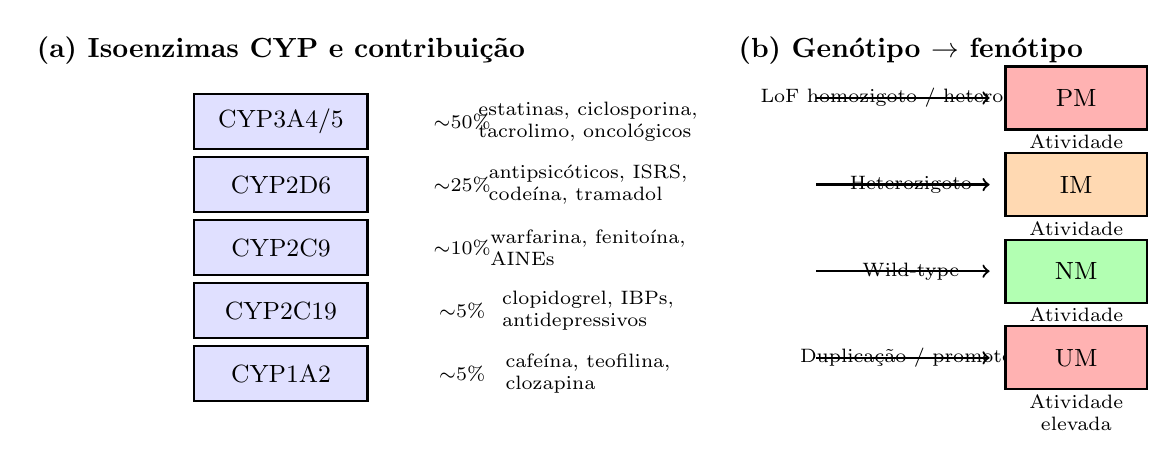
\begin{tikzpicture}[
  every node/.style={font=\small, align=center},
  cyp/.style={rectangle, draw=black, thick, minimum width=2.2cm, minimum height=0.7cm, fill=blue!12},
  fen/.style={rectangle, draw=black, thick, minimum width=1.8cm, minimum height=0.8cm, fill=orange!20},
  seta/.style={->, thick}
]
% Painel esquerdo: contribuição das isoenzimas
\node[font=\bfseries] at (-3.5, 3.7) {(a) Isoenzimas CYP e contribuição};
\node[cyp] (cyp3a4) at (-3.5, 2.8) {CYP3A4/5};
\node[cyp] (cyp2d6) at (-3.5, 2.0) {CYP2D6};
\node[cyp] (cyp2c9) at (-3.5, 1.2) {CYP2C9};
\node[cyp] (cyp2c19) at (-3.5, 0.4) {CYP2C19};
\node[cyp] (cyp1a2) at (-3.5, -0.4) {CYP1A2};
\node[font=\scriptsize] at (-1.2, 2.8) {\(\sim\)50\%};
\node[font=\scriptsize] at (-1.2, 2.0) {\(\sim\)25\%};
\node[font=\scriptsize] at (-1.2, 1.2) {\(\sim\)10\%};
\node[font=\scriptsize] at (-1.2, 0.4) {\(\sim\)5\%};
\node[font=\scriptsize] at (-1.2, -0.4) {\(\sim\)5\%};
\node[font=\scriptsize, align=left] at (0.4, 2.8) {estatinas, ciclosporina,\\tacrolimo, oncológicos};
\node[font=\scriptsize, align=left] at (0.4, 2.0) {antipsicóticos, ISRS,\\codeína, tramadol};
\node[font=\scriptsize, align=left] at (0.4, 1.2) {warfarina, fenitoína,\\AINEs};
\node[font=\scriptsize, align=left] at (0.4, 0.4) {clopidogrel, IBPs,\\antidepressivos};
\node[font=\scriptsize, align=left] at (0.4, -0.4) {cafeína, teofilina,\\clozapina};

% Painel direito: fenótipos metabólicos
\node[font=\bfseries] at (4.5, 3.7) {(b) Genótipo \(\rightarrow\) fenótipo};
\node[font=\scriptsize, align=center] at (4.5, 3.1) {LoF homozigoto / heterozigoto};
\draw[seta] (3.3, 3.1) -- (5.5, 3.1);
\node[fen, fill=red!30] (pm) at (6.6, 3.1) {PM};
\node[font=\scriptsize, align=center] at (6.6, 2.4) {Atividade\\mínima};
\node[font=\scriptsize, align=center] at (4.5, 2.0) {Heterozigoto};
\draw[seta] (3.3, 2.0) -- (5.5, 2.0);
\node[fen, fill=orange!30] (im) at (6.6, 2.0) {IM};
\node[font=\scriptsize, align=center] at (6.6, 1.3) {Atividade\\reduzida};
\node[font=\scriptsize, align=center] at (4.5, 0.9) {Wild-type};
\draw[seta] (3.3, 0.9) -- (5.5, 0.9);
\node[fen, fill=green!30] (nm) at (6.6, 0.9) {NM};
\node[font=\scriptsize, align=center] at (6.6, 0.2) {Atividade\\normal};
\node[font=\scriptsize, align=center] at (4.5, -0.2) {Duplicação / promotor};
\draw[seta] (3.3, -0.2) -- (5.5, -0.2);
\node[fen, fill=red!30] (um) at (6.6, -0.2) {UM};
\node[font=\scriptsize, align=center] at (6.6, -0.9) {Atividade\\elevada};
\end{tikzpicture}
\caption{Farmacogenômica do citocromo P450. (a) Contribuição relativa das principais isoenzimas hepáticas CYP ao metabolismo dos fármacos em uso clínico: CYP3A4/5 (\(\sim\)50\%), CYP2D6 (\(\sim\)25\%), CYP2C9 (\(\sim\)10\%), CYP2C19 (\(\sim\)5\%) e CYP1A2 (\(\sim\)5\%) respondem, em conjunto, por mais de 70\% dos fármacos metabolizados. (b) Tradução genótipo-fenótipo: polimorfismos \emph{loss-of-function} (LoF) determinam fenótipos PM (\emph{Poor Metabolizer}) com atividade mínima, heterozigose resulta em IM (\emph{Intermediate Metabolizer}) com atividade reduzida, genótipo selvagem em NM (\emph{Normal Metabolizer}) e duplicações gênicas ou variantes promotoras em UM (\emph{Ultra-rapid Metabolizer}). As frequências populacionais desses fenótipos variam substancialmente entre grupos étnicos --- CYP2D6 PM é cerca de 5--10\% em europeus e \(\sim\)1\% em asiáticos orientais, enquanto CYP2D6 UM pode atingir 20--30\% em populações do norte da África e Oriente Médio --- com implicações clínicas diretas para ajuste de dose e seleção de fármacos alternativos.}
\label{fig:13-cyp}
\end{figure}

O clopidogrel --- pró-fármaco antiagregante plaquetário amplamente utilizado na prevenção de eventos trombóticos após implante de \emph{stent} coronariano --- oferece um caso paradigmático da relevância clínica desses polimorfismos. O clopidogrel é, em si, farmacologicamente inativo: requer ativação hepática por CYP2C19 para gerar seu metabólito ativo, que bloqueia irreversivelmente o receptor P2Y$_{12}$ plaquetário e inibe a agregação. Polimorfismos \emph{loss-of-function} em CYP2C19 --- notadamente os alelos *2 (c.681G>A, rs4244285) e *3 (c.636G>A, rs4986893) --- reduzem ou abolam essa ativação, com consequências clínicas diretas. Metabolizadores pobres para CYP2C19 apresentam níveis plasmáticos do metabólito ativo cerca de um terço menores que metabolizadores normais, com redução proporcional da inibição plaquetária --- e, em metanálises de estudos clínicos, risco aproximadamente três vezes maior de eventos cardiovasculares maiores (morte cardiovascular, infarto, trombose de \emph{stent}) em usuários de clopidogrel. O alelo *17 (rs12248560), por outro lado, é uma variante promotora que aumenta a atividade de CYP2C19; metabolizadores ultra-rápidos apresentam ativação acelerada do clopidogrel e, paradoxalmente, podem ter risco aumentado de sangramento, embora a magnitude desse efeito seja mais controversa. As implicações práticas, incorporadas em diretrizes de sociedades cardiovasculares norte-americanas e europeias, são: para pacientes CYP2C19 PM/IM, preferir prasugrel ou ticagrelor (alternativas que não dependem de CYP2C19 para sua ativação, ou que dele dependem apenas parcialmente); para pacientes NM/EM, manter clopidogrel como opção custo-efetiva; e para pacientes UM, considerar monitoramento mais cuidadoso. Testes farmacogenômicos para CYP2C19 estão comercialmente disponíveis há mais de uma década, mas a sua implementação sistemática permanece irregular --- reflexo, em parte, da lacuna genérica entre evidência farmacogenômica e sua incorporação em protocolos clínicos.


A descoberta e a validação de \emph{biomarcadores} --- características mensuráveis que indicam processos biológicos normais, patológicos ou respostas a intervenções terapêuticas --- constituem a segunda vertente da medicina personalizada contemporânea. Os biomarcadores podem ser classificados, segundo seu uso clínico, em cinco categorias operacionais. Os biomarcadores \emph{diagnósticos} detectam a presença ou ausência de uma doença; são o exemplo clássico os ensaios imunoenzimáticos para anticorpos anti-HIV, ou os testes moleculares para variantes de CFTR na fibrose cística. Os biomarcadores \emph{prognósticos} preveem a evolução natural de uma doença --- recorrência, progressão, sobrevida --- independentemente de tratamento; o nível sérico de PSA no câncer de próstata é um exemplo, embora controverso por seu perfil de falsos positivos. Os biomarcadores \emph{preditivos} indicam a probabilidade de resposta a uma terapia específica; a presença de mutações ativadoras em EGFR no câncer de pulmão de células não pequenas prediz resposta a gefitinibe e erlotinibe. Os biomarcadores \emph{farmacodinâmicos} medem o efeito biológico de uma intervenção; a queda na carga viral de HIV após início da terapia antirretroviral é um marcador farmacodinâmico de eficácia. Os biomarcadores de \emph{segurança} detectam toxicidade; troponina cardíaca elevada durante tratamento com antraciclinas sinaliza cardiotoxicidade em curso.

O pipeline de descoberta de biomarcadores tem, na era multi-ômica, uma estrutura relativamente padronizada. Parte-se de uma fase de descoberta (\emph{discovery}), em que se aplicam técnicas de alto rendimento --- sequenciamento de RNA, espectrometria de massas, arrays de metabólitos --- a coortes bem caracterizadas de casos e controles, identificando candidatos cuja abundância ou padrão difere significativamente entre os grupos. Os candidatos passam então por uma fase de verificação (\emph{verification}) em coortes independentes, com métodos analíticos otimizados para cada candidato individualmente, e subsequentemente por qualificação (\emph{qualification}) em ensaios prospectivos desenhados especificamente para o biomarcador. Apenas após validação em múltiplas coortes e em contextos clínicos diversos o biomarcador atinge maturidade para implementação em rotina. A taxa de sucesso da fase de descoberta para a fase de implementação é notavelmente baixa --- menos de um por cento dos candidatos identificados em varreduras multi-ômicas chegam à clínica ---, e os gargalos mais significativos estão na reprodutibilidade entre laboratórios e na validação em populações representativas da diversidade étnica e clínica dos pacientes atendidos.

A \emph{estratificação de pacientes} --- classificação em subgrupos com base em características moleculares, clínicas ou demográficas, para tratamento personalizado --- depende criticamente de métodos computacionais capazes de identificar padrões em dados de alta dimensionalidade. O conjunto de dados típico envolve dezenas a centenas de pacientes e milhares a dezenas de milhares de variáveis (expressão de genes, concentrações de proteínas, níveis de metabólitos, variantes genéticas), constituindo o regime de $p \gg n$ (muitas variáveis para poucos pacientes) que desafia a estatística clássica. As técnicas de análise multivariada --- análise de componentes principais (PCA), que projeta os dados em direções de máxima variância; métodos de clustering como K-\emph{means} e clustering hierárquico, que particionam pacientes em grupos com perfis similares; e métodos de fatorização de matrizes não-negativas (NMF), que decompõem os dados em assinaturas latentes --- são o ferramental padrão para essa tarefa. O clustering K-\emph{means}, em particular, tem a vantagem de simplicidade e interpretabilidade: cada paciente é atribuído ao centroide mais próximo no espaço de features, e a partição resultante pode ser visualizada em projeções de baixa dimensionalidade obtidas por PCA ou \emph{t-SNE}. A Seção~\ref{sec:13-exercicios} apresenta um exercício guiado de clustering em dados clínicos simulados, permitindo ao leitor experimentar o método diretamente.

A integração multiômica --- combinando genômica, transcriptômica, proteômica, metabolômica e dados clínicos em modelos preditivos unificados --- representa o estado da arte em estratificação. Métodos como a fatorização conjunta de matrizes (jNMF), redes de correlação multivariadas e abordagens baseadas em autoencoders conseguem identificar subtipos de pacientes que não seriam aparentes em nenhuma camadaômica isolada. O exemplo mais robusto continua sendo o do câncer de mama, mas aplicações estão se multiplicando em oncologia de tumores sólidos, em doenças autoimunes e em doenças neurodegenerativas.

Os diagnósticos baseados em ômicas já constituem uma parcela significativa do armamentário clínico contemporâneo. No campo dos testes genômicos, o sequenciamento de painel de genes é rotina em oncologia --- identifica mutações driver em dezenas a centenas de genes simultaneamente, guiando a escolha de terapias-alvo. O sequenciamento de exoma (WES) e o genoma completo (WGS) são reservados para casos selecionados, especialmente em doenças raras e em oncogenética. A biópsia líquida --- detecção de DNA tumoral circulante (\emph{ctDNA}) no plasma --- permite monitorar carga tumoral, detectar recorrência e identificar mecanismos de resistência sem necessidade de biópsia tecidual invasiva. No campo transcriptômico, três testes para câncer de mama --- Oncotype DX (avalia 21 genes), MammaPrint (avalia 70 genes) e Prosigna/PAM50 (avalia 50 genes classificados em subtipos intrínsecos) --- tornaram-se padrão de cuidado para decidir necessidade de quimioterapia adjuvante em câncer de mama inicial receptor hormonal positivo. Outros perfis transcriptômicos estão em desenvolvimento ou já aprovados para câncer de pulmão, linfomas e leucemias. No campo proteômico e metabolômico, painéis de citocinas e perfis metabolômicos são cada vez mais usados em doenças autoimunes, em erros inatos do metabolismo e em medicina de precisão para diabetes.


A subclassificação molecular do câncer de mama --- consolidada com o advento do painel PAM50 --- oferece um dos exemplos mais bem estabelecidos da substituição da classificação puramente clínica por uma taxonomia molecular. Aproximadamente quinze a vinte por cento dos cânceres de mama superexpressam o receptor HER2 (também chamado ERBB2), uma tirosina-quinase transmembrana cuja ativação constitutiva dirige proliferação celular descontrolada. Outros sessenta a setenta por cento são positivos para receptor de estrogênio (ER) e/ou receptor de progesterona (PR), com perfis proliferativos variados. Aproximadamente quinze por cento são negativos para os três marcadores (triplo-negativos). O painel PAM50, baseado no perfil de expressão de cinqüenta genes classificados por Parker e colaboradores em 2009, identifica cinco subtipos moleculares intrínsecos que reorganizam essa classificação. O subtipo \emph{luminal A} --- receptor de estrogênio positivo, HER2 negativo, Ki67 baixo --- tem o melhor prognóstico e responde adequadamente a hormonioterapia isolada, sem necessidade de quimioterapia adjuvante em muitos casos. O subtipo \emph{luminal B} --- receptor de estrogênio positivo, mas com Ki67 elevado e/ou HER2 positivo --- tem prognóstico intermediário e geralmente se beneficia de hormonioterapia combinada com quimioterapia. O subtipo \emph{HER2-enriquecido} --- receptor de estrogênio negativo, mas HER2 positivo --- responde a terapias anti-HER2 (trastuzumab, pertuzumab, T-DM1, trastuzumab-deruxtecana), tipicamente combinadas com quimioterapia. O subtipo \emph{basal-símile} --- triplo-negativo, com perfil de expressão semelhante a células basais/mioepiteliais --- tem o pior prognóstico e exige quimioterapia citotóxica; novos tratamentos incluem inibidores de PARP para tumores com mutações BRCA1/2 e imunoterapia para tumores com alta carga mutacional ou PD-L1 positivo. A implicação clínica, hoje rotineira, é que pacientes com o mesmo diagnóstico histológico --- ``carcinoma ductal invasivo'', por exemplo --- recebem terapêuticas completamente diferentes dependendo do subtipo molecular, e que a decisão terapêutica sem o painel molecular é considerada, na prática contemporânea, incompletamente fundamentada. A Figura~\ref{fig:13-pam50} apresenta os quatro subtipos principais e seus marcadores canônicos.

\begin{figure}[ht]
\centering
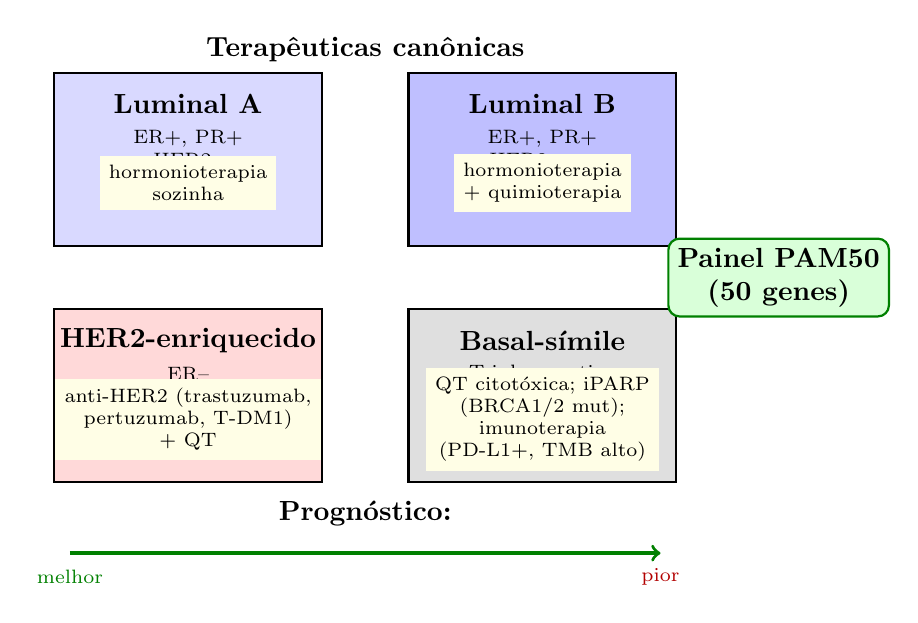
\begin{tikzpicture}[
  every node/.style={font=\small, align=center},
  sub/.style={rectangle, draw=black, thick, minimum width=3.4cm, minimum height=2.2cm},
  marc/.style={font=\scriptsize, align=center}
]
\node[sub, fill=blue!15] (lumA) at (0, 0) {};
\node[font=\bfseries] at (0, 0.7) {Luminal A};
\node[marc] at (0, 0.0) {ER+, PR+\\HER2--\\Ki67 baixo};
\node[sub, fill=blue!25] (lumB) at (4.5, 0) {};
\node[font=\bfseries] at (4.5, 0.7) {Luminal B};
\node[marc] at (4.5, 0.0) {ER+, PR+\\HER2+ ou\\Ki67 alto};
\node[sub, fill=red!15] (her2) at (0, -3.0) {};
\node[font=\bfseries] at (0, -2.3) {HER2-enriquecido};
\node[marc] at (0, -3.0) {ER--\\HER2++\\Ki67 alto};
\node[sub, fill=gray!25] (basal) at (4.5, -3.0) {};
\node[font=\bfseries] at (4.5, -2.3) {Basal-símile};
\node[marc] at (4.5, -3.0) {Triplo-negativo\\(ER--, PR--, HER2--)\\KRT5+, KRT17+};

\node[font=\bfseries] at (2.25, -4.5) {Prognóstico:};
\draw[->, very thick, green!50!black] (-1.5, -5.0) -- (6.0, -5.0);
\node[font=\scriptsize, green!50!black] at (-1.5, -5.3) {melhor};
\node[font=\scriptsize, red!70!black] at (6.0, -5.3) {pior};

\node[font=\bfseries] at (2.25, 1.4) {Terapêuticas canônicas};
\node[font=\scriptsize, align=center, fill=yellow!10] at (0, -0.3) {hormonioterapia\\sozinha};
\node[font=\scriptsize, align=center, fill=yellow!10] at (4.5, -0.3) {hormonioterapia\\+ quimioterapia};
\node[font=\scriptsize, align=center, fill=yellow!10] at (0, -3.3) {anti-HER2 (trastuzumab,\\pertuzumab, T-DM1)\\+ QT};
\node[font=\scriptsize, align=center, fill=yellow!10] at (4.5, -3.3) {QT citotóxica; iPARP\\(BRCA1/2 mut);\\imunoterapia\\(PD-L1+, TMB alto)};

\node[font=\bfseries, fill=green!15, draw=green!50!black, thick, rounded corners] at (7.5, -1.5) {Painel PAM50\\(50 genes)};
\end{tikzpicture}
\caption{Subtipos moleculares de câncer de mama segundo o painel PAM50 (Parker et al., 2009). Os quatro subtipos intrínsecos --- \emph{Luminal A}, \emph{Luminal B}, \emph{HER2-enriquecido} e \emph{Basal-símile} --- reorganizam a classificação histológica tradicional com base em perfis de expressão de cinqüenta genes classificados por similaridade a linhagens celulares de referência. Marcadores canônicos: \emph{Luminal A} (ER+, PR+, HER2--, Ki67 baixo) responde a hormonioterapia sozinha; \emph{Luminal B} (ER+, HER2+ e/ou Ki67 alto) requer hormonioterapia combinada com quimioterapia; \emph{HER2-enriquecido} (HER2 superexpressado) responde a terapias anti-HER2 (trastuzumab, pertuzumab, T-DM1) combinadas com quimioterapia; \emph{Basal-símile} (triplo-negativo) é tratado com quimioterapia citotóxica, e mais recentemente com inibidores de PARP em tumores com mutações BRCA1/2 ou imunoterapia em tumores com alta carga mutacional ou expressão de PD-L1. A seta horizontal indica a gradação de prognóstico, do melhor (\emph{Luminal A}) ao pior (\emph{Basal-símile}).}
\label{fig:13-pam50}
\end{figure}

A seleção de tratamento baseada em perfil molecular estende-se, hoje, a dezenas de indicações oncológicas. No câncer de pulmão de células não pequenas, mutações ativadoras em EGFR (especialmente deleções no exon 19 e a mutação L858R no exon 21) indicam uso de inibidores de tirosina-quinase como erlotinibe, gefitinibe ou osimertinibe (este último ativo também contra a mutação de resistência T790M). Rearranjos envolvendo o gene ALK (resultantes de inversões ou translocações cromossômicas) indicam uso de crizotinibe ou ceritinibe. No melanoma, a mutação BRAF V600E --- presente em cerca de cinqüenta por cento dos melanomas cutâneos --- indica uso de vemurafenibe ou dabrafenibe, frequentemente combinados com inibidores de MEK (trametinibe, cobimetinibe) para prevenir resistência. Na leucemia mieloide crônica, a translocação t(9;22) que gera o gene de fusão BCR-ABL é o evento fundador da doença e o alvo do imatinibe --- paradigma inicial de toda a era das terapias-alvo moleculares. No câncer de mama, mutações em BRCA1/2 indicam sensibilidade a inibidores de PARP (olaparibe, talazoparibe) por inativação de vias alternativas de reparo de DNA. A lista cresce anualmente, e a identificação de novas mutações driver e novas classes de inibidores é uma das áreas mais dinâmicas da oncologia contemporânea.

Os \emph{digital twins} --- já introduzidos no contexto dos ensaios clínicos na Seção~\ref{sec:13-farmacos} --- merecem detalhamento adicional no contexto da medicina personalizada. Um digital twin em sentido pleno é uma réplica computacional individualizada do paciente, construída a partir de três camadas de informação. A primeira camada é \emph{ômica} e compreende dados genômicos (variantes raras e comuns), transcriptômicos (perfil de expressão gênica em tecidos relevantes), proteômicos (níveis de proteínas circulantes e teciduais), metabômicos (perfis de metabólitos) e, cada vez mais, metagenômicos (composição do microbioma). A segunda camada é \emph{fisiológica} e compreende parâmetros clínicos rotineiros --- idade, sexo, peso, função renal e hepática, comorbidades, medicações concomitantes --- além de dados de imagem (ressonância magnética, tomografia, ecocardiograma) e de monitoramento longitudinal (glicemia contínua em diabéticos, pressão arterial em hipertensos, função pulmonar em asmáticos). A terceira camada é \emph{computacional} e compreende os modelos matemáticos que processam essas informações: modelos PBPK já discutidos, modelos de redes regulatórias estimados a partir de dados transcriptômicos, modelos de evolução tumoral calibrados por biópsias seriadas, e, quando aplicável, modelos de resposta imune. A integração dessas três camadas em uma única plataforma computacional, executável para um paciente específico, é o que define o digital twin em sentido estrito --- e é também o que o torna tecnicamente exigente.

A aplicação clínica de digital twins permanece, em 2025, mais promissora do que consolidada, mas resultados parciais começam a aparecer na literatura. Em cardiologia, modelos computacionais individualizados do coração --- integrando imagem por ressonância magnética, medidas hemodinâmicas e genômica --- têm sido usados para planejar procedimentos de ablação e para predizer risco de arritmias em pacientes com cardiopatias congênitas. Em oncologia, projetos-piloto em câncer de próstata utilizam biópsias líquidas seriadas para calibrar modelos de evolução tumoral sob pressão de tratamento hormonal, com o objetivo de antecipar resistência e ajustar terapia. Em diabetes, modelos do pâncreas endócrino, integrando parâmetros de secreção de insulina e sensibilidade periférica, estão sendo explorados como suporte a decisões sobre combinação de agentes e ajuste de doses. A aceitação regulatória, no entanto, exige níveis de evidência e validação que a medicina personalizada computacional ainda não atingiu em escala --- e essa é uma fronteira ativa de pesquisa clínica e de bioestatística.

Os desafios da medicina personalizada não são apenas técnicos --- são também éticos, sociais e organizacionais. Do ponto de vista técnico, permanecem gargalos significativos: a interpretação de variantes de significado incerto (VUS), a integração de dados ômicos heterogêneos em pipelines reprodutíveis, a necessidade de validação prospectiva de biomarcadores em coortes independentes, a padronização de ensaios entre laboratórios, e o custo ainda elevado de sequenciamento e de análise computacional. Do ponto de vista ético e social, três conjuntos de questões se destacam. O primeiro é \emph{privacidade}: dados genômicos são inerentemente identificáveis, podem revelar informações sobre familiares não-consentidos, e expõem os indivíduos a riscos de discriminação por seguradoras, empregadores e até sistemas judiciários. O segundo é \emph{equidade}: o acesso a tecnologias de medicina personalizada é profundamente desigual entre países, entre sistemas de saúde e entre grupos socioeconômicos dentro de um mesmo país --- e há risco real de que a medicina de precisão aprofunde, em vez de reduzir, disparidades existentes em saúde. O terceiro é \emph{capacitação}: tanto profissionais de saúde quanto pacientes precisam de formação específica para compreender, comunicar e decidir sobre testes moleculares --- e essa formação ainda é incipiente na maioria dos currículos médicos e de educação em saúde. A implementação responsável da medicina personalizada exige, portanto, não apenas avanço técnico, mas também frameworks regulatórios atualizados, políticas públicas de equidade e programas de educação em escala.


\section{Aplicações Clínicas}
\label{sec:13-aplicacoes}

Os princípios da medicina de sistemas discutidos nas seções anteriores --- módulos de doença, farmacogenômica, biomarcadores, estratificação molecular, digital twins --- adquirem concreção plena quando aplicados a estudos de caso específicos. Esta seção examina quatro domínios em que a biologia de sistemas já produziu impacto clínico mensurável: a terapia-alvo em oncologia mamária com trastuzumab, o reposicionamento e a modelagem em doenças infecciosas, a resistência a antibióticos como problema sistêmico, e a imunologia de sistemas aplicada à imunoterapia do câncer e à terapia celular com CAR-T.

O câncer de mama HER2-positivo e o desenvolvimento do trastuzumab constituem, juntos, o primeiro sucesso emblemático da medicina personalizada em oncologia e o protótipo de toda uma geração de terapias-alvo que se seguiu. HER2 (do inglês \emph{Human Epidermal growth factor Receptor 2}, também chamado ERBB2 ou NEU) é um receptor tirosina-quinase transmembrana pertencente à família EGFR. Em condições fisiológicas, sua ativação depende de dimerização com outro receptor HER e dispara vias de sinalização --- MAPK/ERK, PI3K/AKT, JAK/STAT --- que regulam proliferação, sobrevivência e diferenciação celular. Em aproximadamente quinze a vinte por cento dos cânceres de mama invasivos, o gene ERBB2 encontra-se amplificado --- frequentemente com mais de seis cópias por célula ---, levando à superexpressão do receptor na superfície celular, à ativação constitutiva de suas vias de sinalização e a um fenótipo clínico agressivo, com taxas de recorrência elevadas e sobrevida reduzida. Antes do desenvolvimento de terapias anti-HER2, o prognóstico dessas pacientes era substancialmente pior que o das pacientes com tumores HER2-negativos.

O trastuzumab --- anticorpo monoclonal humanizado aprovado pela FDA em 1998 e comercializado com o nome Herceptin --- é a primeira terapêutica desenhada especificamente contra HER2 superexpressado. Seu mecanismo de ação combina dois modos complementares: por um lado, liga-se ao domínio extracelular de HER2 e bloqueia sua dimerização e ativação constitutiva, atenuando as vias proliferativas; por outro, recruta células do sistema imune --- células NK e macrófagos --- que mediam citotoxicidade celular dependente de anticorpo (ADCC), amplificando o efeito antitumoral por meio imunológico. Ensaios clínicos pivotais --- em particular o estudo HERA, com mais de cinco mil pacientes randomizadas para receber trastuzumab adjuvante ou observação após cirurgia --- demonstraram redução aproximada de cinqüenta por cento no risco de recorrência e de mortalidade em pacientes com câncer de mama inicial HER2-positivo, com impacto na sobrevida global que permanece evidente em seguimentos de mais de dez anos. O impacto clínico do trastuzumab é, portanto, um dos mais expressivos já registrados para uma terapia-alvo em oncologia, e estabeleceu o paradigma para dezenas de outras terapias desenhadas contra alvos moleculares identificados em subpopulações tumorais.

A obrigatoriedade do teste de HER2 --- realizado rotineiramente por imuno-histoquímica ou por hibridização in situ fluorescente --- em todos os casos de câncer de mama invasivo é, hoje, parte indissociável do protocolo diagnóstico. A estratificação molecular do tumor não é opcional nem tardia; ela precede e determina a decisão terapêutica. Esta é, talvez, a lição metodológica mais importante do caso HER2/trastuzumab: a identificação de um alvo molecular em uma fração significativa da doença --- e a demonstração de que pacientes com esse alvo se beneficiam especificamente de uma terapia desenhada contra ele --- transforma a prática clínica de modo irreversível. Os desenvolvimentos subsequentes --- pertuzumab (anticorpo contra um epitopo distinto de HER2), trastuzumab-deruxtecana (conjugado anticorpo-fármaco com carga útil de inibidor de topoisomerase I), trastuzumab-duocarmazina, e diversos inibidores de tirosina-quinase de pequena molécula como lapatinibe, tucatinibe e neratinibe --- representam a continuação dessa linha de desenvolvimento, cada um com indicações específicas dentro do subgrupo HER2-positivo e cada um contribuindo para refinamento adicional da estratificação.

A medicina de sistemas oferece, ao caso HER2/trastuzumab, uma camada de interpretação adicional que vai além da simples identificação do alvo. A análise de redes mostra que HER2 ocupa posição de nó central (\emph{hub}) em uma sub-rede de sinalização proliferativa que inclui também EGFR, HER3, PI3K, AKT, mTOR e ciclinas D --- e que a eficácia do trastuzumab depende, em parte, do estado de outras proteínas dessa rede (especialmente PI3K e PTEN). Pacientes com mutações ativadoras em PIK3CA ou com perda de PTEN apresentam resposta reduzida ao trastuzumab e podem se beneficiar de combinações com inibidores de PI3K (alpelisibe) ou de mTOR (everolimo). Essa observação ilustra como a biologia de sistemas transforma a decisão terapêutica de uma lógica binária --- HER2 positivo ou negativo --- para uma lógica contínua, na qual o estado de toda a sub-rede é considerado. A Figura~\ref{fig:13-trastuzumab} apresenta o alvo, os mecanismos de ação do anticorpo e a sub-rede HER2 central para a decisão clínica.

\begin{figure}[ht]
\centering
\begin{tikzpicture}[
  every node/.style={font=\small, align=center},
  recpt/.style={rectangle, draw=black, thick, minimum width=1.6cm, minimum height=0.7cm, fill=red!15},
  prot/.style={ellipse, draw=black, thick, minimum width=1.4cm, minimum height=0.7cm, fill=blue!12, inner sep=1pt},
  ab/.style={rectangle, draw=black, thick, minimum width=1.8cm, minimum height=0.7cm, fill=yellow!30},
  ef/.style={font=\scriptsize, align=center, fill=green!10, inner sep=2pt},
  seta/.style={->, thick},
  block/.style={-|, very thick, red!70!black}
]
% Domínio extracelular HER2
\node[font=\bfseries] at (0, 4.0) {Célula tumoral HER2+};
\draw[thick] (-2.5, 1.5) -- (-2.5, 3.5);
\node[recpt, fill=red!25] (her2) at (0, 2.7) {HER2\\ERBB2};
\node[recpt, fill=red!15] (her3) at (3.2, 2.7) {HER3};
\draw[thick] (-2.5, 1.5) -- (4.5, 1.5);
\node[font=\bfseries] at (0, 0.7) {Sub-rede de sinalização};
\node[prot] (pi3k) at (-1.5, 0.0) {PI3K};
\node[prot] (akt) at (0.5, 0.0) {AKT};
\node[prot] (mtor) at (2.5, 0.0) {mTOR};
\node[prot] (mapk) at (4.5, 0.0) {MAPK/ERK};
\draw[seta] (pi3k) -- (akt);
\draw[seta] (akt) -- (mtor);
\draw[seta] (akt.north) to[bend right=20] (mapk.north);
\draw[seta] (her2.south) -- (-1.0, 1.5);
\draw[seta] (her3.south) -- (0.5, 1.5);
% Trastuzumab
\node[ab] (trast) at (-3.5, 3.5) {Trastuzumab\\(Herceptin)};
\draw[block] (trast.east) -- (her2.west);
% ADCC
\node[ef] at (4.0, 3.5) {ADCC:\\NK + macrófagos};
\draw[->, thick, dashed, green!50!black] (trast.north) to[bend left=30] (4.0, 3.5);
% Efeitos antitumorais
\node[font=\bfseries] at (0, -1.2) {Efeitos antitumorais};
\node[ef, fill=blue!10] at (-3.0, -1.7) {Bloqueio de\\dimerização HER2};
\node[ef, fill=blue!10] at (0, -1.7) {Inibição de\\sinalização PI3K/AKT};
\node[ef, fill=blue!10] at (3.0, -1.7) {Citotoxicidade\\imune (ADCC)};
\end{tikzpicture}
\caption{Trastuzumab: alvo, mecanismos de ação e sub-rede HER2. O trastuzumab é um anticorpo monoclonal humanizado que se liga ao domínio extracelular de HER2 (ERBB2) com dois efeitos antitumorais complementares. Primeiro, bloqueia a dimerização de HER2 com outros receptores da família EGFR --- notadamente HER3 ---, atenuando a sinalização proliferativa via PI3K/AKT/mTOR e MAPK/ERK. Segundo, recruta células do sistema imune inato --- células NK e macrófagos --- que medeiam citotoxicidade celular dependente de anticorpo (ADCC), amplificando o efeito antitumoral por via imunológica. A sub-rede HER2 inclui ainda moduladores cuja alteração afeta a resposta clínica: perda de PTEN ou mutações ativadoras em PIK3CA reduzem a resposta e indicam combinação com inibidores de PI3K (alpelisibe) ou mTOR (everolimo). Ensaios clínicos pivotais --- em particular o estudo HERA --- demonstraram redução aproximada de 50\% no risco de recorrência e de mortalidade em pacientes HER2-positivo, com seguimento de mais de dez anos.}
\label{fig:13-trastuzumab}
\end{figure}

O segundo domínio de aplicação é o das \emph{doenças infecciosas}, onde a biologia de sistemas tem contribuído em quatro frentes. A primeira é a caracterização de redes moleculares do patógeno: a análise de redes metabólicas de Mycobacterium tuberculosis, Plasmodium falciparum, Trypanosoma cruzi e outros patógenos de relevância para a saúde brasileira identificou enzimas essenciais --- nós cuja deleção é letal para o patógeno --- e enzimas redundantes --- cuja inibição pode ser compensada ---, permitindo priorizar alvos para desenvolvimento de novos antimicrobianos. A segunda frente é o estudo de interações patógeno-hospedeiro: mapas de interação proteína-proteína entre proteínas virais e humanas, como o construído para SARS-CoV-2 em 2020, identificam mecanismos de subversão da maquinaria celular pelo patógeno e sugerem alvos terapêuticos que podem ser modulados por fármacos já aprovados --- abrindo caminho para reposicionamento. A terceira frente é a caracterização de assinaturas imunes de resposta: perfis transcriptômicos de células imunes em pacientes com tuberculose, leishmaniose ou malária permitem distinguir estágios latente e ativo, prever progressão e identificar pacientes que se beneficiarão de imunoterapia adjuvante. A quarta frente é o desenho racional de vacinas: a vacinologia de sistemas --- uso de abordagens ômicas para identificar antígenos protetores e prever imunogenicidade --- foi decisiva para o desenvolvimento acelerado das vacinas mRNA contra COVID-19.

A tuberculose merece atenção específica por sua relevância global --- estima-se que um quarto da população mundial esteja infectada com Mycobacterium tuberculosis, e que cerca de um décimo desses infectados desenvolverá doença ativa durante a vida --- e por ser exemplo de doença na qual a biologia de sistemas está sendo aplicada de modo integrado. A rede metabólica reconstruída do bacilo inclui mais de setecentas reações enzimáticas, e sua análise in silico permite identificar reações cuja interrupção comprometeria o crescimento do patógeno em diferentes condições (intracelular versus extracelular, em presença ou ausência de oxigênio). Simultaneamente, o estudo transcriptômico de granulomas --- as estruturas teciduais organizadas que o sistema imune forma para conter a infecção --- revela heterogeneidade metabólica e fenotípica das bactérias no interior do granuloma, com subpopulações metabolicamente ativas, dormentes e em replicação lenta coexistindo no mesmo tecido. Essa heterogeneidade é, em parte, responsável pela resistência bacteriana intrínseca aos fármacos tuberculostáticos convencionais --- rifampicina, isoniazida, pirazinamida, etambutol --- e pela necessidade de regimes terapêuticos prolongados (seis meses para tuberculose sensível, até dois anos para tuberculose multirresistente). A biologia de sistemas oferece, nesse contexto, ferramentas para desenvolver novos compostos ativos contra populações bacterianas metabolicamente distintas e para desenhar regimes de combinação que cubram simultaneamente essas populações.


A resistência a antimicrobianos é uma das maiores ameaças à saúde global no século XXI e ilustra, de modo particularmente nítido, como um problema biológico --- a evolução de populações bacterianas sob pressão seletiva --- pode ser abordado pela biologia de sistemas. Os mecanismos de resistência são múltiplos e compreendem mutações em alvos de fármacos (RNA polimerase, subunidades ribossomais, enzimas da via do folato), superexpressão de bombas de efluxo que expulsam o antibiótico da célula, produção de enzimas inativadoras como as $\beta$-lactamases (que hidrolisam o anel $\beta$-lactâmico de penicilinas e cefalosporinas), modificação enzimática do alvo (metilação do rRNA 23S que confere resistência a macrolídeos), e formação de biofilmes que conferem tolerância ao reduzir a penetração do fármaco e criar nichos metabólicos quiescentes. Cada um desses mecanismos é, isoladamente, tratável por meio de fármacos específicos --- inibidores de $\beta$-lactamases como clavulanato e tazobactam restauram a eficácia de amoxicilina e piperacilina; inibidores de bombas de efluxo revertem resistência em algumas cepas --- mas a evolução bacteriana frequentemente acumula múltiplos mecanismos em uma única cepa, gerando perfis de multirresistência que desafiam o armamentário terapêutico convencional.

A biologia de sistemas oferece duas contribuições conceituais importantes para o problema. A primeira é a análise de redes de resistência: grafos nos quais genes de resistência, plasmídeos, elementos móveis e espécies bacterianas constituem os nós, conectados por arestas representando transferência horizontal de genes ou co-ocorrência em isolados clínicos. A análise desses grafos revela que genes de resistência a diferentes classes de antibióticos --- por exemplo, resistência a $\beta$-lactâmicos e a aminoglicosídeos --- frequentemente co-localizam em cassettes gênicos (\emph{integrons}) que se transferem em bloco entre bactérias, explicando por que a multirresistência emerge rapidamente em ambientes hospitalares. A segunda contribuição é o conceito de \emph{collateral sensitivity}: o fenômeno, inicialmente contraintuitivo, pelo qual o desenvolvimento de resistência a um antibiótico A em uma população bacteriana torna essa mesma população mais sensível a outro antibiótico B. Mapeamento sistemático de redes de collateral sensitivity em painéis de cepas bacterianas --- em particular Escherichia coli, Staphylococcus aureus e Pseudomonas aeruginosa --- tem identificado pares e trios de antibióticos que, usados em esquemas de alternância ou de combinação, podem suprimir a evolução de resistência ou mesmo revertê-la.

A imunoterapia do câncer --- uso do sistema imune do próprio paciente para eliminar células tumorais --- é outro domínio em que a biologia de sistemas tem contribuído decisivamente. As estratégias atualmente em uso clínico incluem: inibidores de checkpoint imune --- anticorpos monoclonais contra PD-1 (pembrolizumabe, nivolumabe), PD-L1 (atezolizumabe, durvalumabe) e CTLA-4 (ipilimumabe), que bloqueiam sinais inibitórios das células T e restauram sua capacidade de atacar o tumor; células T com receptor de antígeno quimérico (CAR-T), que são geneticamente modificadas para expressar um receptor sintético contra um antígeno tumoral específico; vacinas terapêuticas contra antígenos tumorais; e vírus oncolíticos que infectam e lisam células tumorais. A taxa de resposta global a inibidores de checkpoint é, hoje, de aproximadamente vinte a quarenta por cento nos cânceres onde estão aprovados --- melanoma, pulmão de células não pequenas, rim, bexiga, carcinoma hepatocelular, linfoma de Hodgkin, entre outros ---, com respostas duradouras em uma fração substancial dos respondedores. Esses números são expressivos, mas deixam claro que a maioria dos pacientes não se beneficia: a identificação de biomarcadores preditivos robustos --- e a compreensão dos mecanismos de resistência primária e adquirida --- é uma das fronteiras mais ativas da oncologia atual.

A imunologia de sistemas --- aplicação de técnicas computacionais e de redes ao estudo do sistema imune --- tem contribuído para a imunoterapia em três frentes. A primeira é a caracterização do microambiente tumoral: perfis transcriptômicos de biópsias tumorais revelam um espectro contínuo entre tumores ``quentes'' (com infiltrado imune denso, citocinas Th1, alta expressão de PD-L1) e ``frios'' (pouco infiltrados, pouco reconhecidos pelo sistema imune), e essa classificação prediz resposta a inibidores de checkpoint. A segunda frente é a identificação de assinaturas de resposta: estudos em larga escala identificaram carga mutacional tumoral (TMB), expressão de PD-L1, assinatura de genes de interferon-$\gamma$, e perfil de células T infiltrantes como biomarcadores com valor preditivo independente, cuja combinação em escores multivariados melhora a predição sobre qualquer marcador isolado. A terceira frente é a modelagem da dinâmica da resposta imune: modelos matemáticos de interação célula T-célula tumoral, calibrados por dados clínicos, informam regimes de dose, frequência e combinação de imunoterapias.

A terapia com células CAR-T --- células T do paciente geneticamente modificadas \emph{ex vivo} para expressar um receptor sintético que reconhece um antígeno tumoral específico --- sintetiza várias das ferramentas discutidas neste capítulo. O processo começa pela coleta (leucaférese) de células T do paciente, segue pela modificação genética por vetor viral (tipicamente lentiviral) que introduz o gene do CAR, expansão \emph{ex vivo} das células modificadas, e reinfusão no paciente após quimioterapia linfodepletora de condicionamento. As células CAR-T, uma vez reinfundidas, proliferam, migram para o tumor, reconhecem as células tumorais via domínio de ligação do CAR, desencadeiam ativação e expansãoclonal e matam as células alvo por mecanismos citotóxicos. Os sucessos clínicos mais expressivos têm sido em neoplasias hematológicas de células B --- leucemia linfoblástica aguda refratária e linfoma difuso de grandes células B ---, com taxas de remissão completa superiores a oitenta por cento em algumas indicações pediátricas. Os efeitos adversos, no entanto, são significativos: síndrome de liberação de citocinas (CRS) e neurotoxicidade associada a células imunes (ICANS) podem ser graves e exigem manejo especializado.

A modelagem computacional tem papel crescente no desenvolvimento de terapias CAR-T. Modelos de dinâmica CAR-T versus tumor predizem expansão inicial, contração e persistência, e identificam regimes de dose que maximizam eficácia sem saturação de citocinas. Modelos de toxicidade simulam o curso temporal de CRS e informam pontos de intervenção com anticorpos anti-IL-6 (tocilizumabe). Modelos de design de CARs de próxima geração --- incorporando co-estimulação adicional (CARs de terceira geração), CARs com citocinas integradas (\emph{armored}), ou lógicas de reconhecimento de múltiplos antígenos --- são usados para iterar projetos antes da síntese experimental, acelerando o ciclo de desenvolvimento. Esse fluxo --- modelo, predição, síntese, validação experimental --- é o ciclo virtuoso da biologia de sistemas aplicada ao desenvolvimento terapêutico.

A pandemia de COVID-19, declarada em março de 2020 e que se estendeu formalmente até maio de 2023, foi a primeira grande crise sanitária global enfrentada em condições de biologia de sistemas madura --- e a primeira em que a abordagem sistêmica contribuiu em todas as frentes de modo integrado. A genômica viral --- sequenciamento rápido e compartilhamento global de genomas --- permitiu rastrear a emergência e a evolução de variantes em tempo quase real, identificar a proteína Spike como alvo vacinal prioritário e atualizar formulações conforme o aparecimento de variantes de escape imune. O reposicionamento de fármacos --- análise computacional de redes de interação SARS-CoV-2-hospedeiro --- identificou compostos candidatos em questão de semanas, alguns dos quais (remdesivir, dexametasona, baricitinibe) foram subsequentemente validados em ensaios clínicos. A caracterização transcriptômica de resposta imune --- estudos como o consórcio \emph{Human Cell Atlas} --- identificou assinaturas de progressão para doença grave, em particular o perfil de ``tempestade de citocinas'' com IL-6, TNF e quimiocinas elevadas. A modelagem epidemiológica --- integrada a dados de mobilidade, testagem e hospitalização --- guiou políticas de distanciamento social e previu o impacto de intervenções não-farmacêuticas. O desenvolvimento de vacinas --- a tecnologia de mRNA, com décadas de pesquisa fundamental prévia, demonstrou nesse contexto sua capacidade de projeto racional, síntese química em escala industrial e desenvolvimento clínico acelerado. Menos de um ano separou o sequenciamento do SARS-CoV-2 da autorização das primeiras vacinas mRNA, uma escala de tempo sem precedentes na história da vaccinologia e uma demonstração concreta do poder da abordagem sistêmica em saúde pública.


\section{Exercícios}
\label{sec:13-exercicios}

Esta seção apresenta um conjunto de exercícios que cobrem os principais conceitos discutidos no capítulo, com ênfase em modelagem matemática, análise de redes e integração de dados multi-ômicos. Os exercícios de modelagem farmacocinética podem ser resolvidos analiticamente e por simulação computacional em Python, usando funções da biblioteca \texttt{SciPy} (\texttt{odeint} para integração de sistemas de equações diferenciais, \texttt{scipy.optimize} para ajuste de parâmetros). Os exercícios de redes utilizam a biblioteca \texttt{networkx} para construção, manipulação e análise de grafos. O exercício de clustering recorre ao \texttt{scikit-learn} (\texttt{KMeans}, \texttt{StandardScaler}, \texttt{PCA}). O projeto integrador ao final convida o leitor a combinar todas essas ferramentas em um pipeline coerente de análise de dados de câncer.

\textbf{Exercício 1 (Modelo farmacocinético de um compartimento).} Um paciente recebe dose intravenosa em bolus de 500 mg de um fármaco cujo volume de distribuição é $V_d = 50$ L e cuja meia-vida de eliminação é $t_{1/2} = 4$ h. Calcule (a) a constante de eliminação $k_e$, (b) o clearance do fármaco, (c) a concentração plasmática após 8 horas da administração, e (d) a área sob a curva (AUC) total. Em seguida, implemente o modelo em Python e gere um gráfico da concentração plasmática em função do tempo entre $t=0$ e $t=24$ h, com linha de referência horizontal indicando a meia-vida. Comente o efeito de uma redução de 50\% no volume de distribuição sobre a concentração inicial e sobre o tempo em que a concentração cai a um quarto da inicial.

\textbf{Exercício 2 (Modelo de dois compartimentos).} Implemente um modelo farmacocinético de dois compartimentos em Python usando \texttt{odeint} para integração numérica. Use os parâmetros $k_e = 0{,}15$ h$^{-1}$, $k_{12} = 0{,}30$ h$^{-1}$, $k_{21} = 0{,}20$ h$^{-1}$, dose de 1000 mg administrada por via intravenosa no compartimento central, $V_1 = 30$ L e $V_2 = 20$ L. Simule a evolução temporal das concentrações nos compartimentos central e periférico durante 48 horas. Identifique visualmente as duas fases da curva: distribuição rápida inicial e eliminação terminal. Calcule a concentração no estado de equilíbrio (\emph{steady-state}) se a mesma dose total for administrada por infusão contínua durante 24 horas. Compare com a concentração média em um regime de doses múltiplas orais administradas a cada 6 horas, assumindo biodisponibilidade oral de 80\%.

\textbf{Exercício 3 (Análise de rede fármaco-alvo).} Considere o seguinte grafo bipartido de interações fármaco-alvo: o fármaco A liga-se aos alvos T1, T2 e T3; o fármaco B liga-se aos alvos T2 e T4; o fármaco C liga-se aos alvos T3, T4 e T5. (a) Construa a matriz de adjacência do grafo usando \texttt{networkx}. (b) Calcule o grau de cada fármaco na rede --- número de alvos aos quais se liga --- e o grau de cada alvo --- número de fármacos que se ligam a ele. (c) Identifique alvos compartilhados entre pares de fármacos (T2 compartilhado por A e B; T3 compartilhado por A e C; T4 compartilhado por B e C) e discuta o que essa sobreposição implica em termos de potencial para efeitos adversos comuns entre os fármacos. (d) Sugira candidatos a reposicionamento com base na sobreposição de alvos: quais outros compostos com perfil de alvos similar poderiam ser eficazes em indicações adjacentes? (e) Calcule o coeficiente de clustering e a centralidade de \emph{betweenness} dos nós e comente quais alvos e fármacos ocupam posições estruturalmente mais importantes na rede.

\textbf{Exercício 4 (Detecção de módulos de doença).} Carregue uma rede de interação proteína-proteína de uma base como \texttt{STRING} restrita a proteínas associadas a doença cardiovascular (genes de risco derivados de GWAS Catalog). Aplique o algoritmo de Louvain (\texttt{networkx.community.louvain\_communities}) ou Girvan-Newman para detectar comunidades (módulos) na rede. Interprete funcionalmente cada módulo usando enriquecimento de termos Gene Ontology --- por exemplo, módulo enriquecido em ``resposta imune inata'', módulo enriquecido em ``metabolismo lipídico'', módulo enriquecido em ``sinalização de insulina''. Compare os módulos detectados com módulos de doenças relacionadas --- diabetes tipo 2, obesidade, hipertensão --- e comente o grau de sobreposição observado. Discuta como essa sobreposição fornece uma explicação molecular para comorbidades cardiovasculares-metabólicas.

\textbf{Exercício 5 (Farmacogenômica do CYP2D6 e codeína).} Um paciente é metabolizador pobre (PM) para CYP2D6 e recebe codeína --- pró-fármaco opióide convertido em morfina por CYP2D6 --- para manejo de dor pós-operatória. (a) Preveja o efeito da condição de PM sobre o manejo da dor: a analgesia esperada será maior, menor ou equivalente à de um metabolizador normal? (b) Recomende ajuste de dose ou medicação alternativa: codeína em dose padrão seria adequada, deve-se aumentar a dose, ou seria melhor substituir por um opióide que não dependa de CYP2D6 para sua ativação (como morfina diretamente)? (c) Formule uma explicação ao paciente sobre a importância do teste farmacogenômico: como comunicar que uma diferença herdada em um único gene pode afetar a eficácia de um analgésico, sem criar ansiedade desnecessária nem transmitir determinismo exagerado? (d) Liste outros fármacos comumente prescritos metabolizados por CYP2D6 (antidepressivos, antipsicóticos, betabloqueadores) para os quais o resultado do teste farmacogenômico deste paciente teria implicações práticas.

\textbf{Exercício 6 (Estratificação molecular de câncer de mama).} Implemente clustering K-\emph{means} em um conjunto de dados de expressão gênica de câncer de mama (use o dataset público TCGA-BRCA disponível via \texttt{TCGAbiolinks} em R, ou um dataset simulado com perfis conhecidos). Normalize os dados, aplique redução de dimensionalidade por PCA para visualização, execute K-\emph{means} com $k = 4$ (correspondente aos subtipos PAM50 principais) e visualize os clusters em projeção bidimensional. Compare os clusters obtidos com os subtipos clínicos conhecidos (Luminal A, Luminal B, HER2-enriquecido, Basal-símile) --- avalie concordância por métricas como índice de Rand ajustado. Identifique os genes mais discriminantes de cada cluster e comente sua relevância biológica (por exemplo, ESR1 e PGR no Luminal A; ERBB2 no HER2-enriquecido; KRT5 e KRT17 no Basal-símile).

\textbf{Projeto integrador (Análise de dados clínicos multi-ômicos).} Implemente um pipeline completo de análise de dados multi-ômicos de pacientes com câncer. As etapas propostas são: (1) download de dados de expressão gênica, mutações somáticas e dados clínicos de um repositório público (TCGA, cBioPortal ou GEO), com filtragem de variantes raras e genes de baixa variância; (2) pré-processamento com normalização adequada ao tipo de dado (DESeq2 ou \texttt{limma} para expressão, filtragem por frequência alélica para mutações); (3) análise exploratória com PCA, \emph{heatmaps} e clustering hierárquico; (4) estratificação com K-\emph{means} ou NMF para identificar subgrupos moleculares; (5) análise diferencial entre subgrupos identificados, identificando genes, vias e assinaturas enriquecidas; (6) curvas de Kaplan-Meier por subgrupo com teste log-rank; (7) validação em coorte independente (METABRIC ou ICGC); (8) interpretação biológica por enriquecimento funcional em Gene Ontology, KEGG e Reactome; (9) discussão crítica das implicações clínicas: os subgrupos identificados correspondem a diferenças terapêuticas conhecidas? Há subgrupos com pior prognóstico que poderiam se beneficiar de terapias específicas? O entregável final é um relatório técnico contendo código comentado em R ou Python, figuras, tabelas sumárias e interpretação clínica das descobertas.

\section{Recapitulação}
\label{sec:13-recapitulacao}

Este capítulo atravessou quatro domínios em que a biologia de sistemas se encontra com a prática médica contemporânea, articulando teoria --- redes biológicas, modelos compartimentais, farmacogenômica, módulos de doença --- com prática clínica --- biomarcadores em uso, ensaios pivotais, fármacos aprovados. Antes de passar aos exercícios, convém consolidar os pontos centrais em uma visão de conjunto, articulada em torno dos cinco eixos da transição paradigmática introduzidos na Seção~\ref{sec:13-introducao}.

O primeiro eixo --- \emph{unidade de análise: da molécula para a rede} --- foi exemplificado em três frentes distintas. Na descoberta de fármacos, a farmacologia de redes (Seção~\ref{sec:13-farmacos}) substitui a lógica ``um fármaco, um alvo, uma doença'' por grafos bipartidos fármaco-alvo em escala genômica, cujas métricas de centralidade, comunidades e sobreposição informam reposicionamento e previsão de efeitos. Na compreensão de doenças, a noção de módulo de doença (Seção~\ref{sec:13-doencas}) sintetiza genes de risco, proteínas e metabólitos em bolas topológicas do interactoma, e a sobreposição entre módulos explica comorbidades sem invocar causas adicionais. Na decisão terapêutica, a sub-rede em torno de HER2 (Seção~\ref{sec:13-aplicacoes}) ilustra como o estado de \emph{toda} a rede de sinalização --- HER2, HER3, PI3K, AKT, mTOR, PTEN --- modula a resposta ao trastuzumab, transformando a decisão binária (positivo/negativo) em decisão contínua (estado de toda a sub-rede).

O segundo eixo --- \emph{causalidade multifatorial} --- aparece com nitidez na farmacogenômica do CYP2C19 (Seção~\ref{sec:13-personalizada}), onde a combinação de genótipo do paciente, classe do fármaco e contexto clínico substitui a causalidade simples da farmacologia clássica. A mesma multifatorialidade estrutura os modelos PBPK, que integram expressão tecidual de transportadores, abundância de isoenzimas CYP, função renal e hepática e comorbidades em uma representação mecanística única.

O terceiro eixo --- \emph{terapêutica combinatória} --- é concretizado nos regimes de combinação que hoje dominam a oncologia: trastuzumab com pertuzumab e quimioterapia, inibidores de BRAF com inibidores de MEK, inibidores de checkpoint com CAR-T, inibidores de PARP com imunoterapia. A farmacologia de redes não é metáfora: é o ferramental que justifica e orienta essas combinações, em contraste com a lógica monofarmacológica do século XX.

O quarto eixo --- \emph{integração multi-ômica} --- aparece nos perfis PAM50 (50 genes) que reorganizam o câncer de mama em subtipos clinicamente acionáveis, nos testes Oncotype DX (21 genes) e MammaPrint (70 genes) que decidem quimioterapia adjuvante, nos painéis genômicos que guiam a escolha de terapias-alvo em câncer de pulmão, melanoma e leucemia, e nos digital twins que aspiram a integrar genômica, transcriptômica, proteômica, metabolômica, metagenômica, imagem e dados clínicos em um modelo computacional individualizado.

O quinto eixo --- \emph{holismo computacional} --- atravessa todo o capítulo como método subjacente. Os modelos compartimentais PK (um e dois compartimentos), os modelos PBPK, os modelos de redes regulatórias subjacentes aos digital twins, os modelos de interação célula T-célula tumoral que informam regimes de imunoterapia e os modelos de evolução clonal que calibram biópsias líquidas seriadas são, todos, exemplos de como a única maneira de capturar a emergência em sistemas complexos é através de modelos matemáticos e simulações --- não de intuições reducionistas sobre componentes isolados.

Do ponto de vista metodológico, três técnicas transversais merecem destaque por reaparecerem em múltiplos contextos. \emph{Clusters e estratificação} --- K-\emph{means}, NMF, clustering hierárquico, PCA, \emph{t}-SNE --- organizam pacientes em subtipos clinicamente relevantes no câncer de mama (PAM50), no diabetes tipo 2 (cinco subtipos), na asma (endotipos) e em doenças neurodegenerativas. \emph{Análise de redes} --- centralidade, comunidades, propagação, sobreposição de módulos --- estrutura a farmacologia de redes, os módulos de doença, as vias de sinalização em torno de alvos terapêuticos e as redes de transferência horizontal de genes de resistência bacteriana. \emph{Modelagem dinâmica} --- equações diferenciais ordinárias, modelos compartimentais, modelos baseados em agentes, redes bayesianas --- formaliza a farmacocinética, a farmacodinâmica, a propagação de sinais, a dinâmica tumoral e a evolução de resistência a antimicrobianos.

Do ponto de vista ético e operacional, três conjuntos de desafios permanecem abertos. O primeiro é a \emph{validação}: a tradução de uma assinatura molecular robusta em um teste clínico padronizado, custo-efetivo, com utilidade prospectiva demonstrada em ensaios clínicos desenhados com estratificação molecular --- processo que ainda consome anos entre a descoberta do biomarcador e sua implementação em rotina. O segundo é a \emph{equidade}: a distribuição desigual de tecnologias de sequenciamento, de capacidade computacional e de cobertura por sistemas de saúde entre países, regiões e grupos socioeconômicos é um determinante estrutural das desigualdades em saúde que a medicina de precisão pode tanto reduzir quanto ampliar, dependendo das escolhas de implementação. O terceiro é a \emph{interpretabilidade}: a comunicação de decisões terapêuticas baseadas em modelos computacionais complexos --- incluindo digital twins --- para pacientes e profissionais de saúde exige interfaces, formação e frameworks regulatórios que ainda estão em construção.

Em síntese, este capítulo procurou mostrar que a medicina de sistemas não substitui a medicina clínica --- incorpora-a, dotando-a de ferramentas quantitativas, preditivas e personalizadas. As redes biológicas, os modelos matemáticos e os dados multi-ômicos são, todos, instrumentos ao serviço da decisão clínica, e o desafio --- técnico, ético, social --- é fazer com que esses instrumentos sejam acessíveis, interpretáveis e úteis para o paciente real, em tempo real, no consultório ou à cabeceira do leito.

\section{Notas Bibliográficas}
\label{sec:13-referencias}

{As referências reunidas nesta seção cobrem o espectro temático do capítulo: medicina de sistemas, descoberta de fármacos e farmacologia de redes, doenças complexas, medicina personalizada e farmacogenômica, biomarcadores e digital twins, imunoterapia e terapia celular. A maioria dos trabalhos citados é de acesso aberto ou está disponível nas bibliotecas digitais das principais universidades. Para aprofundamento sistemático, recomenda-se a leitura dos artigos seminais --- \cite{barabasi2011} para medicina de redes, \cite{hanahan2011} para hallmarks do câncer, \cite{hopkins2008} para farmacologia de redes, \cite{ashley2016} para medicina personalizada, e \cite{auffray2009} para medicina de sistemas --- na ordem em que aparecem no texto. Os livros de Loscalzo e colaboradores e o compêndio de Wolkenhauer oferecem visões integradoras de maior fôlego. Para aplicações computacionais, os artigos sobre clustering em câncer por \cite{brunet2004} e sobre redes de interação por \cite{menche2015} são particularmente instrutivos.

}

\begin{thebibliography}{99}

\bibitem{barabasi2011} Barabási A.L., Gulbahce N., Loscalzo J. (2011). \textit{Network medicine: a network-based approach to human disease}. Nature Reviews Genetics, 12:56--68.

\bibitem{hanahan2011} Hanahan D., Weinberg R.A. (2011). \textit{Hallmarks of cancer: the next generation}. Cell, 144:646--674.

\bibitem{hopkins2008} Hopkins A.L. (2008). \textit{Network pharmacology: the next paradigm in drug discovery}. Nature Chemical Biology, 4:682--690.

\bibitem{menche2015} Menche J., Sharma A., Kitsak M., et al. (2015). \textit{Disease networks: uncovering disease-disease relationships through the incomplete interactome}. Science, 347:1257601.

\bibitem{ashley2016} Ashley E.A. (2016). \textit{Towards precision medicine}. Nature Reviews Genetics, 17:507--522.

\bibitem{auffray2009} Auffray C., Chen Z., Hood L. (2009). \textit{Systems medicine: the future of medical genomics and healthcare}. Genome Medicine, 1:2.

\bibitem{schadt2009} Schadt E.E. (2009). \textit{Molecular networks as sensors and drivers of common human diseases}. Nature, 461:218--223.

\bibitem{zhou2014} Zhou X., Menche J., Barabási A.L., Sharma A. (2014). \textit{Human symptoms-disease network}. Nature Communications, 5:4212.

\bibitem{zhao2012} Zhao S., Iyengar R. (2012). \textit{Systems pharmacology: network analysis to identify multiscale mechanisms of drug action}. Annual Review of Pharmacology and Toxicology, 52:505--521.

\bibitem{csermely2013} Csermely P., Korcsmáros T., Kiss H.J., et al. (2013). \textit{Structure and dynamics of molecular networks: a novel paradigm of drug discovery}. Pharmacology \& Therapeutics, 138:333--408.

\bibitem{roden2015} Roden D.M., McLeod H.L., Relling M.V., et al. (2019). \textit{Pharmacogenomics}. The Lancet, 394:521--532.

\bibitem{chen2012} Chen R., Snyder M. (2013). \textit{Promise of personalized omics to precision medicine}. Wiley Interdisciplinary Reviews: Systems Biology and Medicine, 5:73--82.

\bibitem{brunet2004} Brunet J.P., et al. (2004). \textit{Metagenes and molecular pattern discovery using matrix factorization}. Proceedings of the National Academy of Sciences, 101:4164--4169.

\bibitem{loscalzo2017} Loscalzo J., Barabási A.L., Silverman E.K. (Eds.). (2017). \textit{Network Medicine: Complex Systems in Human Disease and Therapeutics}. Harvard University Press, Cambridge, MA.

\bibitem{hood2011} Hood L., Friend S.H. (2011). \textit{Predictive, personalized, preventive, participatory (P4) cancer medicine}. Nature Reviews Clinical Oncology, 8:184--187.

\bibitem{ideker2012} Ideker T., Krogan N.J. (2012). \textit{Differential network biology}. Molecular Systems Biology, 8:565.

\bibitem{califano2017} Califano A., Alvarez M.J. (2017). \textit{The recurrent architecture of tumour initiation, progression and drug sensitivity}. Nature Reviews Cancer, 17:116--130.

\bibitem{kitano2007} Kitano H. (2007). \textit{A robustness-based approach to systems-oriented drug design}. Nature Reviews Drug Discovery, 6:202--210.

\bibitem{wolkenhauer2013} Wolkenhauer O. (2013). \textit{Systems Medicine}. Springer, New York.

\bibitem{zhu2016} Zhu H., Xia M. (Eds.). (2016). \textit{Advances in Systems Biology}. Springer, New York.

\end{thebibliography}

